% !TEX root = ../../thesis.tex

\section{Building Model \label{sec:building_model}}
%\begin{abstract}
%Commercial buildings are responsible for a large fraction of energy consumption in developed countries, and therefore are targets of energy efficiency programs. Motivated by the large inherent thermal inertia of buildings, the power consumption can be flexibly scheduled without compromising occupant comfort. This temporal flexibility offers opportunities for energy savings and the provision of frequency regulation to support grid stability. To realize these goals, it is of prime importance to identify a realistic model for the temperature dynamics of a building. In this paper, we identify a low-dimensional data-driven model and a high-dimensional physics-based model for the same system at different spatial granularities and temporal seasons using experimental data collected from an entire floor of an office building on the University of California, Berkeley campus. We perform a quantitative comparison in terms of estimates of the inherent thermal gains due to occupancy, open-loop prediction accuracies, and closed-loop control schemes. %Under an energy efficient control scheme, we show that both models result in a similar optimal control strategy, and therefore 
%We conclude that data-driven models could serve as a substitution for highly complex physics-based models with an insignificant loss of prediction accuracy for many applications.
%\end{abstract}


%!TEX root = ../../thesis.tex

\section{Introduction}
\label{sec:Introduction}
%According to \cite{Perez-Lombard:2008aa}, residential and commercial buildings account for up to 40\% of the total electricity consumption in developed countries, with an upward trend. Heating, ventilation and air-conditioning (HVAC) systems are a major source of this consumption \cite{USenergy:2017}. %, ~35% of energy use in commercial buildings is for heating, cooling and ventilation.
%Nevertheless, their power consumption can be flexibly scheduled without compromising occupant comfort, due to the thermal capacity of buildings. As a result, HVAC systems have become the focal point of research, with the goal of utilizing this source of consumption flexibility. From the point of view of energy efficiency, researchers have studied optimization of building control in order to minimize power consumption \cite{Siroky:2011aa, Parisio:2014aa}.  
%More recently, it has been proposed to engage buildings in supporting the supply quality of electricity and the grid stability, by participating in the regulation of electricity's frequency \cite{Balandat:2014contractdesign, Lin:2015exp, Vrettos:2014aggregation, Baccino:2014aa}.
%
%
%All of the above research activities are based on a valid mathematical model describing the thermal behavior of buildings. 

Traditionally, buildings have been modeled with high-dimensional physics-based models such as resistance-capacitance (RC) models \cite{Maasoumy:2014ab, Sun, David, Hao_multizone}, TRNSYS \cite{Duffy:2009aa} and EnergyPlus \cite{Zhao2013EP}. These models are motivated by the thermodynamics of the building and explicitly model the heat transfer between components of the buildings. The advantage of such models is their high granularity of temperature modeling, but a drawback is their high dimensionality which makes them computationally expensive. 
Although there has been extensive work on model reduction, this remains to be a non-trivial task. A large body of this work focuses on linear models, whereas physics-based models for commercial buildings with a variable air volume (VAV) HVAC system are bilinear in nature. Furthermore, existing model reduction techniques often result in a loss of interpretability of states \cite{Dobbs:2012aa} and a significant increase in the model's prediction error \cite{Goyal:2012modelreduction}. 

Motivated by these shortcomings, a new direction of research attempts to identify lower-dimensional, data-driven models, e.g. with Input-Output models \cite{Lin:2015exp} and semiparametric regression \cite{Aswani:2012aa}. The purpose is to alleviate the computational complexity in expense for coarser and less accurate temperature predictions.


%The contribution of this paper is two-fold. First, we aim to improve existing
%data-driven model identification techniques. Unlike \cite{Radecki:2012aa}, \cite{Radecki:2013ab}, who model the evolution of the building's energy consumption without a specific control input, we identify a model for temperature evolution in multiple building zones that is amenable to control design, i.e. with airflows as inputs. Our model also differs from that in \cite{Aswani:2012aa}, which uses HVAC supply air temperature as the single control input, resulting in a simpler identification problem but on the other hand, offers less flexibility in control.

In this chapter, we propose both a physics-based method and a data-driven method to identify models of a multi-zone building, that is easy to implement with the building in regular operation, and captures internal gains such as occupancy, without the need of additional instruments like carbon dioxide sensors.
Our procedures use excitation experiments that actively perturb the building and generate data that can be used for more accurate parameter identification.

More importantly, we perform a \textit{quantitative comparison} of the data-driven and physics-based models in terms of open-loop prediction accuracy and closed-loop control strategies, based on the \textit{same testbed} (the entire floor of an office building). % using \textit{experimental data} collected from the building, as opposed to simulated data. 
We conclude that a low-dimensional data-driven model is suitable for building control applications, such as frequency regulation, due to its minor loss of prediction accuracy compared to high-dimensional physics-based models, but significant gain in computational ease. 
To the best of our knowledge, the extant body of literature has analyzed data-driven and physical models for the identification of temperature evolution in commercial buildings only in an isolated fashion (in particular not on the same testbed) \cite{Ma:2011aa}, \cite{Siroky:2011aa}, \cite{Lin:2015exp}, \cite{Qie}. In addition, some of these models were identified for fictitious buildings with synthetic data \cite{Cole:2013aa, Goyal:2013occupancy, David}, while others used experimental data collected under environments with little or no disturbance, e.g. without occupants \cite{Lin:2015exp}. Our work differs from these existing works in two aspects. First, we use experimental data to identify models for a multi-zone commercial building under regular operation, which is subject to significant disturbances such as occupancy. Second, although the existing literature mentions the differences between data-driven and physics-based models, the prevailing isolationist approach does not provide any quantitative comparison with respect to building control applications - a fact we would like to alleviate by juxtaposing a data-driven with a physics-based model.


%The remainder of this paper is organized as follows: In Section \ref{sec:Preliminaries}, we describe the testbed and the experimental data collected for our research. Section \ref{sec:Data_Driven_Model} presents the identification process for a purely data-driven model with semiparametric regression, followed by Section \ref{sec:Physics_Based_Model}, which details the procedure for identifying a physics-based model. Section \ref{sec:Comparison} then compares the performance of the data-driven model and the physics-based model under open-loop prediction accuracy and closed-loop energy efficient optimal control. We show that, despite the higher accuracy of the complex physics-based model compared to the low-dimensional data-driven model, the optimal control strategies with respect to HVAC operation cost while maintaining the thermal comfort of occupants is almost identical for both systems. We conclude in Section \ref{sec:Conclusion} with a summary of our current and intended future work.


%!TEX root = ../../thesis.tex

\section{Experimental Data}
\label{sec:Preliminaries}


\subsection{Data Collection}\label{sec:exp_data}
We collected 51 weeks of one-minute resolution temperature data for the six zones along with the airflow rates of the 21 VAV boxes, SAT and the outside air temperature from the \textit{simple Measurement and Actuation Profile} (sMAP). sMAP is a protocol that collects, stores and publishes time-series data from a wide variety of sensors \cite{smap, Dawson-Haggerty:2012aa}. The hourly global horizontal solar radiation data was obtained from a nearby weather station \cite{SolarRad}, from which the incidence solar radiation of the four geographic directions was calculated with the \texttt{PV\_LIB} toolbox \cite{pv_model}. All collected data were down-sampled or interpolated, respectively, to 15 minute intervals. 
These 51 weeks of data span periods when the building was under normal operation as well as periods with excitation experiments. 

To increase identifiability of the building model, forced response experiments were performed. These experiments were conducted during Saturdays to (a) minimize effects due to occupancy on our collected data, and thus facilitate subsequent parameter identification; (b) minimize impact to building operation and exploit larger comfort bounds on room temperatures during the weekends. Indeed, the comfort bounds were never violated during the forced experiments. 
%Details on the design of our excitation experiments can be found in \cite{Qie}.
%For accurate parameter identification, temperatures of neighboring zones should not be strongly correlated \cite{Lin_multizone}. 
%For buildings in regular operation, this is generally achievable through forced response experiments. 
Because of commercial buildings' large thermal inertia, each forced excitation must last sufficiently long before temperature changes are observable (we chose 2 hours for our excitation experiment).
More specifically, starting at 8am, the supply air's flow rate to one zone is set to its maximum value every 2 hours. During this 2 hour period, all of its neighboring zones' airflow rates are set to their minimum values, and each of the remaining zones' airflow rate is set to a random value. 
This procedure is repeated for each of the 6 zones. 
%This experiment is performed during weekends as (a) it minimizes effects due to building occupancy on our data, and thus the subsequent parameter identification; (b) temporary violation of comfort constraints during the weekend was allowed.

%For accurate parameter identification, temperatures of neighboring zones should not have strong correlation \cite{Lin_multizone}. Our testbed is a regular office building in operation, thus forced response experiments were performed during Saturdays to (a) increase identifiability of the building model; (b) minimize effects due to occupancy on our data, and thus facilitate subsequent parameter identification; (c) minimize disturbance to building operation \cite{Qie}.


\subsection{Data Splitting}
Next, we defined the seasons ``fall" (early September until mid December), ``winter" (mid December until late January), and ``spring" (late January until mid May) in order to account for different occupancy levels during the fall and spring semesters, and the winter break. After the weeks have been assigned to the seasons, a random portion of the data in each season (e.g. we chose 90\%) was defined as the training data, and the remaining weeks to be removed prior to the analysis were declared as the test set, which were used to assess the accuracy of the building model fitted on the training data.

%\subsection{Notation}
%\label{sec:Notation}
%Let $\hat{\left( \cdot \right)}$ denote either the conditional expectation or the estimated value of a variable. Let $\tilde{\left( \cdot \right)}$ the predicted value of a variable, respectively.

%\qie{I removed bold face for vectors and matrices, because otherwise every equation for the individual zone model and physics based model will be in bold face. Also for notation consistency, I thought about changing the x and v in the physics-based model to T and w, but since it is a state space model, I think it would be clearer to stick to the standard notation for state space models, where x is the state (temperature in this case) and v is the disturbance, so I changed all temperatures to x, and disturbances to v.}

%!TEX root = ../../thesis.tex

\section{Data-Driven Model}
\label{sec:Data_Driven_Model}
We identify a difference equation for the temperature evolution with semiparametric regression, using 51 weeks of experimental data collected from the fourth floor of SDH. Semiparametric regression in buildings has been proposed by \cite{Aswani:2012aa}, where the authors used only one week of historic data to model the temperature evolution and used the HVAC's supply air temperature as the single control input. % including an exogenous heating load that captures the effect of occupancy, electric devices, outside air temperature, and solar radiation. 
We extend this approach by taking into account multiple weeks, which we separate into three seasons (fall, winter, spring) so as to characterize the different levels of the exogenous heating load for different temporal seasons. 
In addition, we model the room temperatures as a function of airflow rates from multiple VAVs to obtain a model which can be used for more sophisticated control strategies.
%We make use of cross-validation across all weeks to find the optimal model, therefore allowing for a more general analysis of the thermal behavior rather than restricting ourselves to identifying a model tailored to a single week, as is done in \cite{Aswani:2012aa}.

Next, we first introduce the semiparametric method using a simple lumped zone model of the fourth floor, and then identify a multi-zone model for the same floor which we will use to make quantitative comparisons with the physics-based model.

\subsection{Lumped Zone}
\label{sec:Lumped_Zone}
\subsubsection{Model Setup}
In order to facilitate analysis, the entire 4th floor of SDH is treated as a single zone, with the scalar temperature $x$ corresponding to the %area-averaged zone 
average temperature on the entire floor and the input $u$ as the sum of the inflow of all 21 VAV boxes. %This lumped model assumes a uniform temperature on the entire floor, $x$, and has been commonly used in literature \cite{Ma:2012aa, Oldewurtel:2010aa}. 
Then, the temperature evolution is assumed to have the following form:
\begin{equation}\label{eq:Temperature_evolution}
x(k+1) = a x(k) + b u(k) + c^\top v(k) + q_{\text{IG}}(k) + \epsilon(k),
\end{equation}
where %$u$ denotes the total air inflow to the entire floor and 
$v := \left[v_\text{Ta}, v_\text{Ts}, v_\text{solE}, v_\text{solN}, v_\text{solS}, v_\text{solW} \right]^\top$ is a vector of known disturbances that describes ambient air temperature, the HVAC system's supply air temperature, and solar radiation from each of the four geographical directions.
In addition, $q_{\text{IG}}$ represents the internal gains due to occupancy and electric devices, and $\epsilon$ denotes independent and identically distributed zero mean noise with constant and finite variance which is conditionally independent of $x$, $u$, $v$, and $q_{\text{IG}}$. Finally, $a$, $b \in \mathbb{R}$ and $c \in \mathbb{R}^6$ are unknown coefficients to be estimated using semiparametric regression \cite{Ruppert:2003aa, Hardle:2000aa}.

\subsubsection{Smoothing of Time Series}
The $q_{\text{IG}}$ term of Equation \eqref{eq:Temperature_evolution} is treated as a nonparametric term, so that \eqref{eq:Temperature_evolution} becomes a partially linear model. By taking conditional expectations on both sides of \eqref{eq:Temperature_evolution}, we obtain

\begin{equation}\label{eq:Conditional_Expectation}
\begin{aligned}
\hat{x}(k+1) &= a\hat{x}(k) + b\hat{u}(k) + c^\top\hat{v}(k) \\
& \quad + \mathbb{E}\left[ q_{\text{IG}}(k) \vert k \right] + \mathbb{E}\left[ \epsilon(k) \vert k \right],\\
\end{aligned}
\end{equation}
\noindent
where the conditional expectations $\hat{x}(\cdot) = \mathbb{E}\left[ x(\cdot) \vert \cdot \right]$, $\hat{u}(\cdot) = \mathbb{E}\left[ u(\cdot) \vert \cdot \right]$, and $\hat{v}(\cdot) = \mathbb{E}\left[ v(\cdot) \vert \cdot \right]$ are used.
Noting that $\mathbb{E}\left[ \epsilon(\cdot) \vert \cdot \right] = 0$ and assuming $\mathbb{E}\left[ q_{\text{IG}}(\cdot) \vert \cdot \right] = q_{\text{IG}}(\cdot)$, subtracting \eqref{eq:Conditional_Expectation} from \eqref{eq:Temperature_evolution} gives
\begin{equation}\label{eq:subtract}
\begin{split}
x(k+1) - \hat{x}(k+1) = a\left( x(k) - \hat{x}(k) \right) \\ + b\left( u(k) - \hat{u}(k) \right)
+ c^\top \left( v(k) - \hat{v}(k) \right) + \epsilon(k).
\end{split}
\end{equation}
The unknown internal gains term has been eliminated, and thus the coefficients $a, b, c$ in \eqref{eq:subtract} can be estimated with any regression method.

The conditional expectations $\hat{x}(\cdot), \hat{u}(\cdot)$ and $\hat{v}(\cdot)$ are obtained by smoothing the respective time series \cite{Aswani:2012aa}. We made use of locally weighted linear regression with a tricube weight function, where we use $k$-fold cross-validation to determine the bandwidth for regression.
%that assigns weights $\psi_i$ 
%\begin{equation}\label{eq:tricube_weight_function}
%\psi_i = \left( 1- \left| \frac{z-z_i}{d(z)} \right|^3 \right)^3, 
%\end{equation}
%that belong to $z_i \in \mathcal{Z}$, which is a neighbor of the data point $z$ to be smoothed along the abscissa within the span $\mathcal{Z}$ (all data points around $z$ taken into account to smooth the time series at $z$), and $d(z)$ the distance from $z$ to the farthest predictor within $\mathcal{Z}$. The width $d(z)$ of the span $\mathcal{Z}$ is determined with $k$-fold cross-validation.
The error measure used for in-sample estimates is the \textit{Root Mean Squared} (RMS) \textit{Error} between the measured temperatures $\bar{x}(k)$ and the model's predicted temperatures $x(k)$ over a time horizon of $N$ steps (e.g. we chose a 24 hour time horizon, $N = 96$):
\begin{equation}\label{eq:RMS}
\text{RMS error} = \left(\frac{1}{N}\textstyle\sum_{k=1}^N \left[\bar{x}(k) - x(k)\right]^2 \right)^{1/2}.
\end{equation}
\subsubsection{Bayesian Constrained Least Squares}
A main challenge in identifying the model is that commercial buildings are often insufficiently excited. Take SDH for example, whose room temperatures under regular operation only vary within a range of 2$^{\circ}$C and inflow of the VAV boxes hardly varies at all. To overcome this, data collected during forced response experiments described in Section \ref{sec:exp_data} was used in training the model. To further compensate for the lack of excitation, a Bayesian regression method is used, which allows our prior knowledge of the building physics to be incorporated in the identification of coefficients. More specifically, Gaussian prior distributions are used for the coefficients $a$ and $b$, i.e., $a \sim \mathcal{N}( \mu_a, \Sigma_a)$ and $b \sim \mathcal{N}( \mu_b, \Sigma_b)$, where $\mathcal{N}( \mu, \Sigma)$ denotes a jointly Gaussian distribution with mean $\mu$ and covariance matrix $\Sigma$. In addition, $a$, $b$ and $c$ are constrained to be identical for the different seasons, since they model the underlying physics of the building which are assumed to be invariant throughout the year. 

Let $\mathcal{T} = \{1, 2, \cdots, N\}$ denote the $N$ weeks of training data (e.g. we chose $N = 45$), and define $\mathcal{F} = \{i \in \mathcal{T} \text{ such that $i$ is a week in fall} \}$ as the set of training weeks from the fall season. Similarly, define the sets of training weeks from the winter and spring as $\mathcal{W}$ and $\mathcal{S}$.
The coefficient identification problem is then formulated as follows:
\begin{equation}\label{eq:data_opt}
\begin{aligned}
(\hat{a}, \hat{b} , \hat{c}) = &\arg\min_{a, b, c}~\left(J_\mathcal{F} + J_\mathcal{W} + J_\mathcal{S}\right) + \Vert \Sigma_a^{-1/2} (a - \mu_a) \Vert^2\\
& \quad\quad + \Vert \Sigma_b^{-1/2} (b - \mu_b)  \Vert^2 \\
\text{s.t.}~ J_\mathcal{X}= & \textstyle \sum_{i \in \mathcal{X}} \Vert x_i(k+1) - \hat{x}_i(k+1) - a\left( x_i(k) - \hat{x}_i(k) \right)\\
& - b\left( u_i(k) - \hat{u}_i(k) \right) - {c}^\top\left( v_i(k) - \hat{v}_i(k) \right) \Vert ^ 2\\
& \text{for } \mathcal{X} \in \lbrace \mathcal{F}, \mathcal{W}, \mathcal{S} \rbrace, \\
& 0 < a < 1,~ b \leq 0,~ c \geq 0. \\
\end{aligned}
\end{equation}
%where subscripts f, w, and s represent fall, winter and spring, respectively. 
In other words, $J_\mathcal{F}$, $J_\mathcal{W}$ and $J_\mathcal{S}$ represent the sum of squared errors between experimentally measured temperatures and model's predicted temperatures for fall, winter and spring, respectively.
The sign constraints on the parameters $b$ and $c$ translate into the fact that the temperature to be estimated positively correlates with all components in $v$ and negatively correlates with the VAV airflow. The range of $a$ is a consequence of Newton's Law of Cooling.
%One problematic aspect that greatly complicates the identification of the coefficients is the little excitation of the system, since the observed temperatures vary within a small range only (e.g. 20-22$^{\circ}$C for fall and spring weeks, and 19-21$^{\circ}$C for the winter weeks) and the inflow of the single VAV boxes hardly vary at all. Contrary to \cite{Aswani:2012aa}, where the authors used Bayesian Linear Regression, which relies on covariance matrices penalizing regularization terms and which are set in a subjective fashion, we use a grid search algorithm coupled with Least Squares approximation to determine the optimal set of parameters $(\hat{a}, \hat{b}, \mathbf{\hat{c}})$ that minimize the sum of the weekly RMS of the individual seasons \eqref{eq:RMS}, with the constraint that $(\hat{a}, \hat{b})$ are identical for the different seasons since it is assumed that the inherent physics of the lumped zone remain unchanged throughout the year. We therefore formulate the problem as follows:
%\begin{equation}\label{eq:grid_search}
%\begin{aligned}
%& \hat{a}, \hat{b} = \arg\min_{a, b}~\left(\text{RMS}_f + \text{RMS}_w + \text{RMS}_s\right) \\
%& \text{s.t.}~\hat{c}_j = \arg\min_{c_j} \Vert T_j(n+1) - \hat{T}_j(n+1) - a\left( T_j(n) - \hat{T}_j(n) \right)\\
%& - b\left( u_j(n) - \hat{u}_j(n) \right) - c_j\left( w_j(n) - \hat{w}_j(n) \right) \Vert
% \\
%& j \in \lbrace\text{fall}, \text{winter}, \text{spring}\rbrace
%\end{aligned}
%\end{equation}
%That is, for a fixed pair of coefficients $(a, b)$, $\mathbf{\hat{c}}_j$ is defined to be the minimizer of the described loss function for season $j$ which we determine with Least Squares fitting. The optimal parameters $\hat{a}, \hat{b}, \mathbf{\hat{c}}$ are therefore the triplet of parameters that minimize the sum of the RMS over all seasons.\\
%Figure \ref{fig:RMS_seasons} shows the RMS for the individual seasons and the mean for different parameters $\left(a, b\right)$ to solve \eqref{eq:grid_search}. It can be seen that the heat maps for the three different seasons exhibit different characteristics. For fall and spring, the optimal value of $a$ appears to be $\approx 0.85$, whereas the RMS in winter period decreases beyond $a>0.85$. The RMS takes a minimum for $a\approx 0.87, b\approx 0.03$. However, the average RMS heat map indicates that the RMS hardly increases for the given range of parameters $a, b$, since the maximum mean RMS exceeds the optimum by $<10\%$ only.
%\begin{figure}[hbtp]
%\centering
%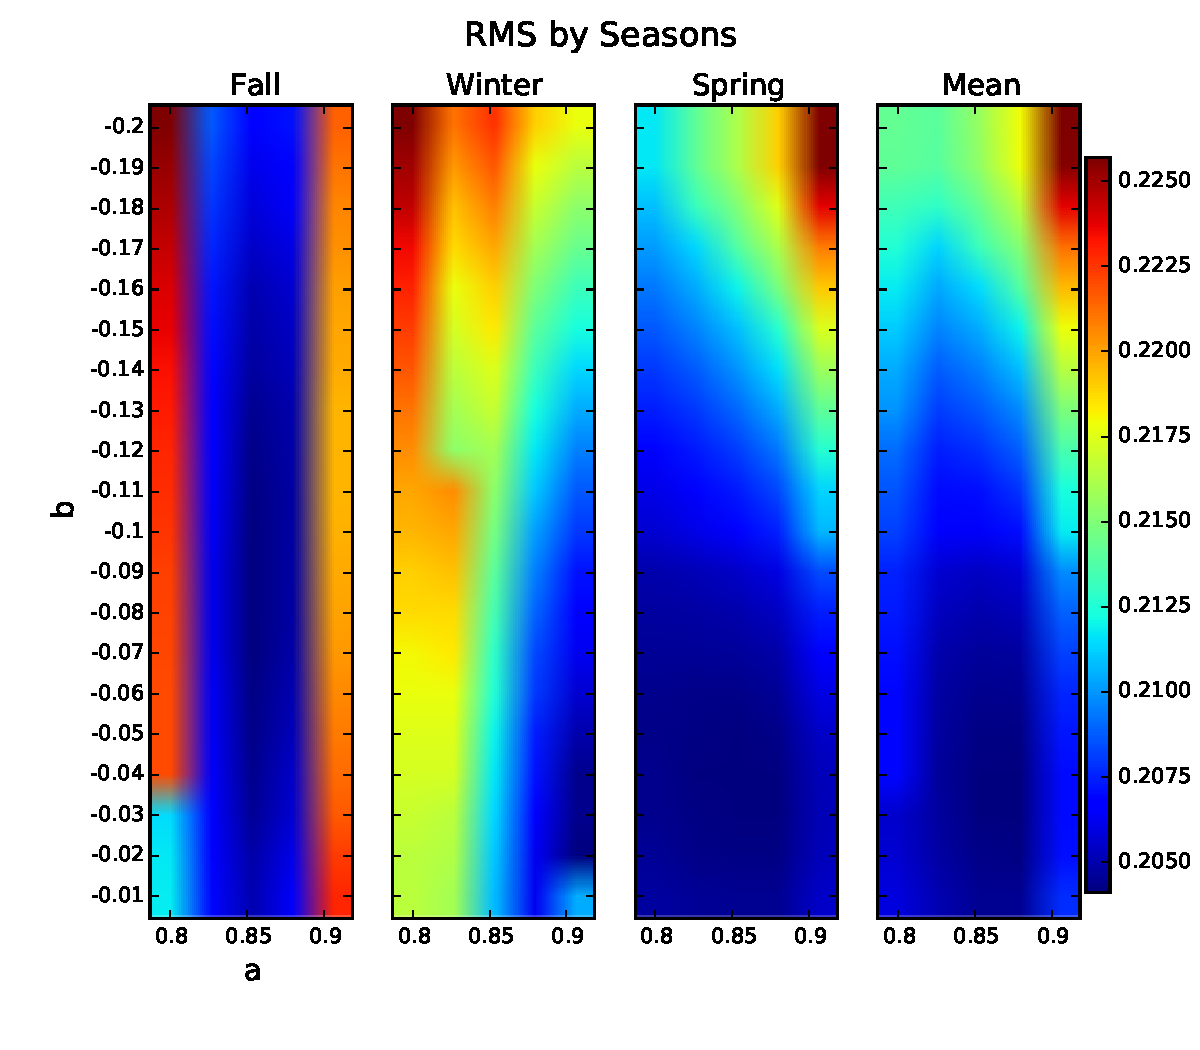
\includegraphics[scale=0.42]{Figures/RMS_cumul.pdf}
%\caption{RMS for different seasons with different $\hat{a}$, $\hat{b}$}
%\label{fig:RMS_seasons}
%\end{figure}
%Without the prior terms, the optimal value $b$ that minimizes the cost function in \eqref{eq:data_opt} is found to be $\approx 0.03$. With the unit of the airflow being $\left[kg/s\right]$, the 15-minute temperature reduction due to an average inflow of $2.2 kg/s$ would only be 0.066$^{\circ}$C.

%Thus, due to the insufficient excitation of the building, we use physical intuition to increase the parameter $b$ from its optimal value $b=0.03$ so as to give the control input more weight without compromising the prediction quality to an unjustifiable extent. 
To find the effect of the VAV inflow on the 15-minute temperature evolution, we computed the 15-minute incremental reductions in temperature $\Delta x$ recorded during the excitation experiments. 
%\footnote{The excitation experiments were carried out on weekends to minimize disruption of building operation. The temperature during these experients were kept within comfort bounds (20-22$^\circ$C).}. 
It is assumed that the large inflow $u$ dominates all other effects such that we can assume
\begin{equation}\label{eq:excitation_equation}
\Delta x = x(k+1) - x(k) = b\cdot u(k)
\end{equation}
for all $k$ during the excitation period. The estimated prior $\mu_b$ can then be isolated from \eqref{eq:excitation_equation}. The prior $\mu_a$ was set as the optimal $\hat{a}$ identified by \eqref{eq:data_opt} without the prior terms. The covariance matrices $\Sigma_a$ and $\Sigma_b$ were chosen subjectively. 
%The result is shown in Figure \ref{fig:decrem_T}. The negative slope of the linear fit corresponds to the prior on $b$. Given this prior $b=-0.18$, we choose the value of $a$ that yields the minimum RMS. Thus, we identify $\hat{a}=0.83, \hat{b} = -0.18$ with a mean RMS of 0.236. 
%\qie{Modify this paragraph to describe choice of prior without figure, and note difference between b value for 1 zone and whole floor, because b depends on the thermal mass of the zone.}
%\begin{figure}[hbtp]
%\centering
%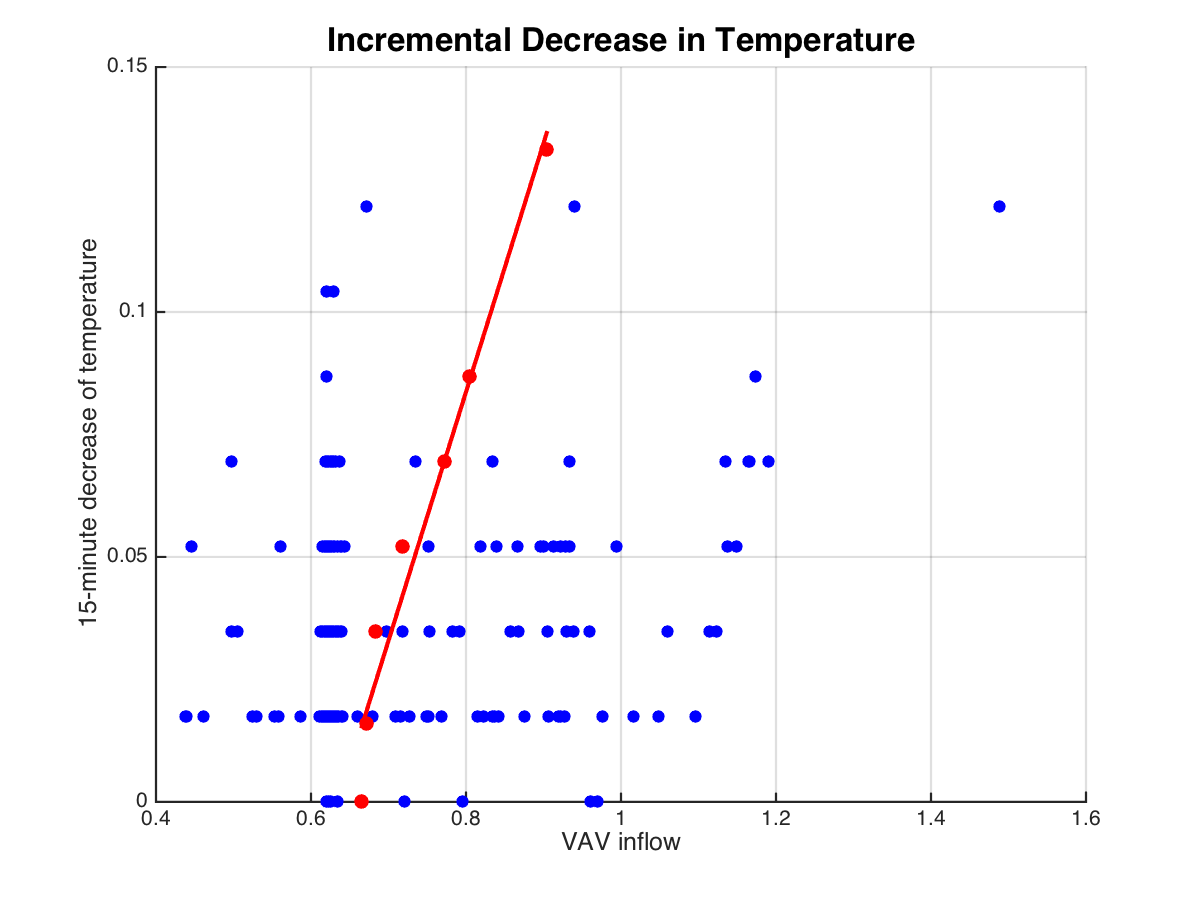
\includegraphics[scale=0.42]{Figures/b_prior.png}
%\caption{Incremental decrease of $T$ due to $u$}
%\label{fig:decrem_T}
%\end{figure}
\subsubsection{Estimation of Internal Gains}
With the estimated coefficients $\hat{a}, \hat{b}, \hat{c}$ in hand, the internal gains $q_{\text{IG}}$ can be estimated by manipulating \eqref{eq:Conditional_Expectation}: 
\begin{equation}\label{eq:qig_estimation}
\hat{q}_{\text{IG}}(k) = \hat{x}(k+1) - \left(\hat{a}\hat{x}(k) + \hat{b}\hat{u}(k) + \hat{c}^\top \hat{v}(k)\right).
\end{equation}
%This can be interpreted as the difference between the smoothed temperature $\hat{x}(k+1)$ and the predicted expected temperature.
%$\mathbb{E}\left[x(k+1)\right]$. \textcolor{red}{(I think this may be what's causing the confusion, because from previous definition $\mathbb{E}\left[x(k+1)\right]$ = $\hat{x}(k+1)$. But this suggests they are different variables. Can we remove this?)} 
%With the estimated parameter coefficients being constant over the different seasons, a distinct function of internal gains is estimated for each season by averaging the estimated weekly gains for a given season.
A distinct function of internal gains is estimated for each season. In other words, \eqref{eq:qig_estimation} is used to estimate an instance of the internal gains function for each week $i$ in the training set $\mathcal{T}$. The internal gains function for each season, $\hat{q}_{\text{IG},\mathcal{X}}$ is then defined as the average of estimated weekly gains for all weeks $i \in \mathcal{X}$ and $\mathcal{X} \in \{ \mathcal{F}, \mathcal{W}, \mathcal{S} \}$.

%From the definition of the temperature model \eqref{eq:Temperature_evolution}, the internal gain at time $k$, overlaid with noise $\epsilon(k)$, could also be estimated as the difference between the measured temperature $\bar{x}(k+1)$ and the predicted temperature $\tilde{x}(k+1)$:
%\begin{equation}\label{eq:qig_observational}
%\hat{q}_{\text{IG}}(k) + \epsilon(k) = \bar{x}(k+1) - \underbrace{\hat{a}\bar{x}(k) - \hat{b}\bar{u}(k) - \hat{c}^\top \bar{v}(k)}_{\tilde{x}(k+1)}.
%\end{equation}

\subsubsection{Results}
The estimated internal gains for each season are shown in Figure \ref{fig:qig_comparison_plot}.
\begin{figure}[hbtp]
\centering
\vspace*{-0.0cm}
\hspace*{-0.6cm}
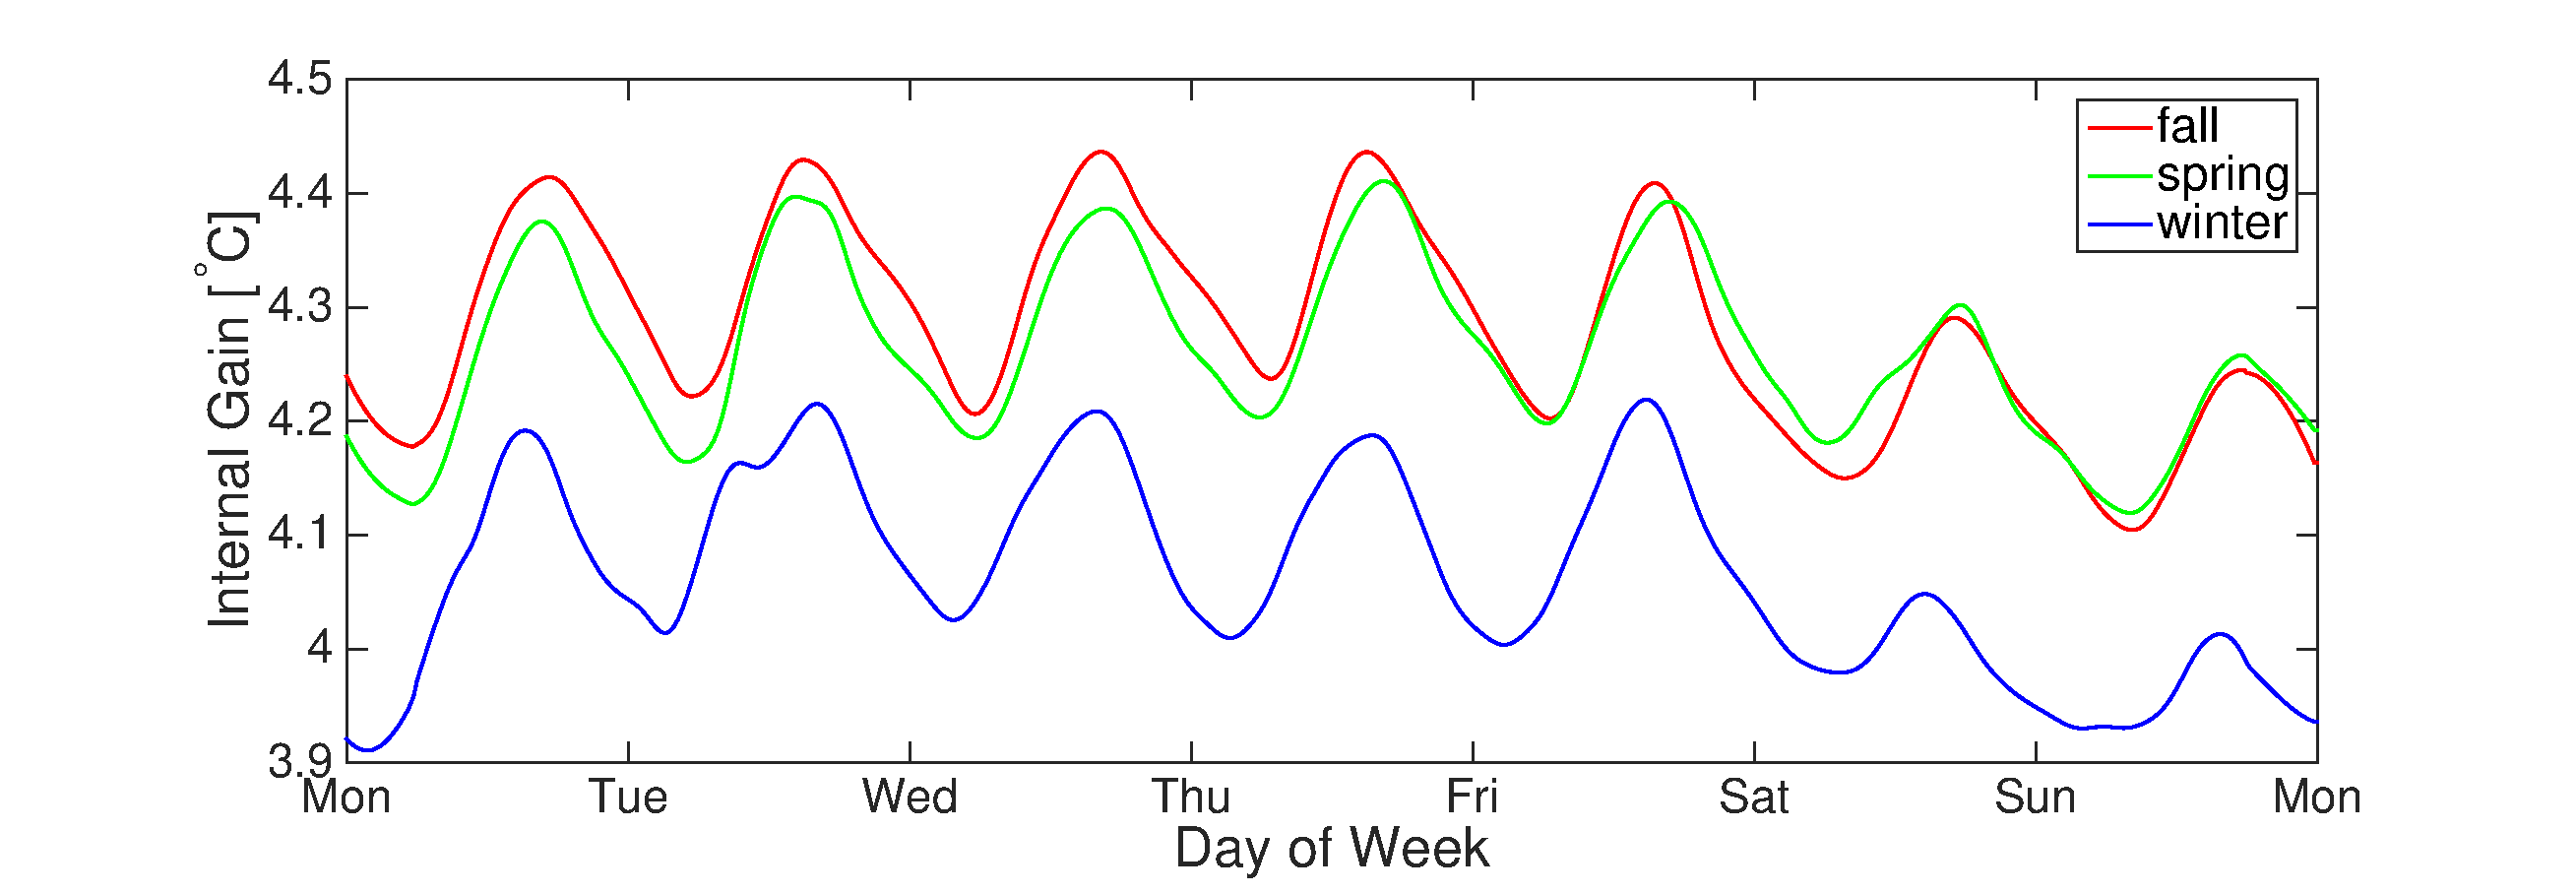
\includegraphics[scale=0.22]{chapters/building_model/figures/data_lump_qig.eps}
\vspace*{-0.3cm}
\caption{Estimated Internal Gain $q_{\text{IG}}$ from the Data-Driven Model by Season, Lumped Case}
\vspace*{-0.3cm}
\label{fig:qig_comparison_plot}
\end{figure}
Observe that, for all three seasons, the internal gains exhibit a daily trend with local peaks around the late afternoon and local minima at night. Moreover, the amplitudes of the internal gains are considerably smaller during the weekends, suggesting a lighter occupancy. It can further be seen that the magnitude of the internal gains is smallest for the winter season, which is in accordance with our intuition since most building occupants are absent during that period.

%Furthermore, computing $q_{\text{IG}}$ with smoothed time series \eqref{eq:qig_estimation} yields smoother results than with \eqref{eq:qig_observational}, since there is no noise term $\epsilon(k)$. This suggests that the difference between the solid and the dashed line represents the zero mean Gaussian noise of \eqref{eq:Temperature_evolution}.

Lastly, since the Bayesian Constrained Least Squares algorithm \eqref{eq:data_opt} has identified a set of parameter estimates $\hat{a}, \hat{b}, \hat{c}$ valid for all three seasons to account for the time-invariant physics of the building, the temperature predictions are of the same nature for all three seasons. We thus conclude that the inherent differences between the seasonal temperature data are captured by the internal gains and can be compared between the seasons on a relative level.

The identified models for the different seasons found with \eqref{eq:data_opt} are
\begin{equation}\label{eq:lumped_zone_res}
\begin{aligned}
x(k+1) & = 0.80\cdot x(k) - 0.18\cdot u(k) \\
 & ~~ + \left[0.0019, 0.028, \mathbf{0} \right] v(k) + q_{\text{IG},\mathcal{X}}(k) \\
 & =  0.80\cdot x(k) - 0.18\cdot u(k) \\
 & ~~ + 0.0019 \cdot v_{\text{Ta}}(k) + 0.028 \cdot v_{\text{Ts}}(k) + q_{\text{IG},\mathcal{X}}(k) \\
 & \text{for } \mathcal{X} \in \lbrace \mathcal{F}, \mathcal{W}, \mathcal{S} \rbrace\\
\end{aligned}
\end{equation}
The estimated coefficients of $c$ corresponding to the solar radiation disturbances are very small ($< 10^{-6}$) compared to the other estimated coefficients. Since the temperatures are of the order $10^{\circ}$C, air inflow around 1 kg/s and solar radiation about 100 W/m$^2$, the effect of solar radiation on the room temperature is orders of magnitude less than that of other factors and hence can be neglected.

The average RMS prediction errors are 0.22$^{\circ}$C, 0.17$^{\circ}$C and 0.23$^{\circ}$C for fall, winter and spring, respectively, showing that our model predicts the temperature reasonably well. 

%Figure \ref{fig:temp_plot_lump} shows a comparison between the actual temperature of the three zones and the predicted temperature with a prediction horizon of $N = 96$ (24 hours) for a selected week of the holdout test data. Note that the predicted temperature is initialized in 24 hour intervals.

%\begin{figure}[hbtp]
%\centering
%\vspace*{-0.31cm}
%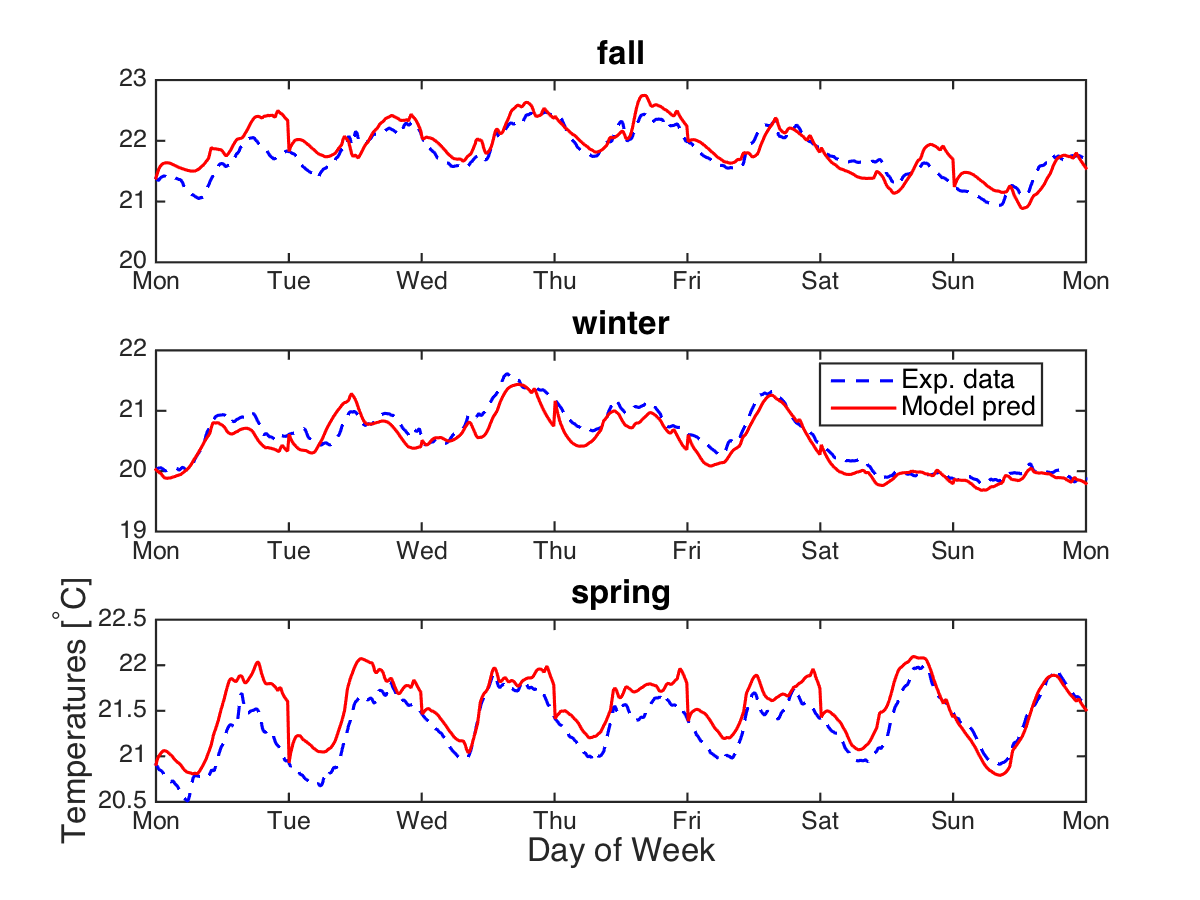
\includegraphics[scale=0.46]{Figures/lumped_test.png}
%\vspace*{-0.7cm}
%\caption{Measured and Predicted Temperatures by Season}
%\label{fig:temp_plot_lump}
%\end{figure}

%Figure \ref{fig:qig_seasons} shows the estimated internal gain for the three seasons fall, winter, and spring identified with \eqref{eq:grid_search} and $\hat{a}=0.83, \hat{b} = -0.18$. 
%\begin{figure}[hbtp]
%\centering
%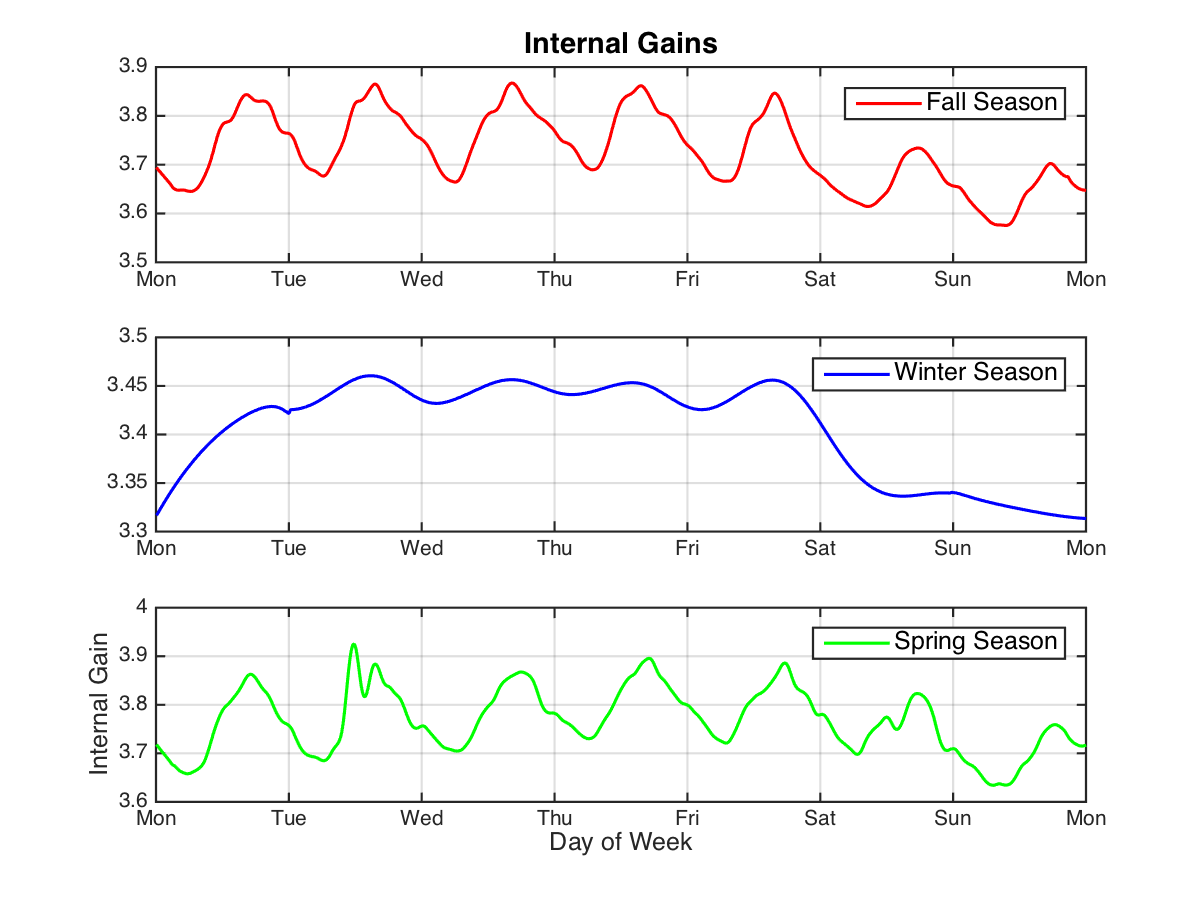
\includegraphics[scale=0.46]{Figures/Internal_gains.png}
%\caption{Estimated internal gains for the seasons, lumped case}
%\label{fig:data_lump_qig}
%\end{figure}
%The models for the different seasons are identified as
%\begin{equation}\label{eq:lumped_zone_res}
%\begin{split}
%T_f(n+1) =& ~0.83\cdot T_f(n) - 0.18\cdot u(n) + \\ &\left[0.0024, 0.0241, \mathbf{0}\right]\cdot w(n) + q_{\text{IG},f}(n) \\
%T_w(n+1) =& ~0.83\cdot T_w(n) - 0.18\cdot u(n) + \\ & \left[0.0185, 0.0186, \mathbf{0}\right]\cdot w(n) + q_{\text{IG},w}(n) \\
%T_s(n+1) =& ~0.83\cdot T_s(n) - 0.18\cdot u(n) + \\ & \left[8\cdot 10^{-10}, 0.0228, \mathbf{0}\right]\cdot w(n) + q_{\text{IG},s}(n)
%\end{split}
%\end{equation}
%In \eqref{eq:lumped_zone_res}, the indices "f", "w", and "s" denote the fall, winter, and spring season, with weekly RMS  0.208, 0.251, 0.250, respectively. The estimated parameters belonging to the known disturbances $w$ are negligible $\left(<1\cdot 10^{-5}\right)$ for the global incidence radiations from the four geographic directions, A possible explanation for these small coefficients could be that the effect of the solar radiation is partially captured by the internal gain $q_{\text{IG}}$. Indeed, we found that the inclusion of a Lasso-regularization term to \eqref{eq:grid_search} shrinks these estimated coefficients $c$ further to zero, with a negligible increase of $q_{\text{IG}}$ and the RMS.\\
%It is important to note that the estimated autoregressive coefficient $\hat{a}$ and the control coefficient $\hat{b}$ have been forced to be identical (equation \eqref{eq:grid_search}), and that the estimated coefficients on the supply air temperature are similar for the three seasons. Further, the estimated coefficient for the outside air temperature has little effect on the temperature evolution. Thus, the only significant difference characterizing seasonal effects is the weekly internal gain, which is shown in Figure \ref{fig:qig_seasons}. The internal gains $q_{\text{IG}}~$ for the different seasons exhibit a daily trend with local peaks around the late afternoon and local minima at night. Moreover, for the fall and spring season, the amplitudes of the internal gain are considerably smaller during the weekend. It can further be seen that the magnitude of the internal gain is smallest for the winter season, which is in accordance with our intuition since most people are absent during that period.\\
\subsection{Individual Zones}\label{sec:Indiv_Zones}
\subsubsection{Model Setup}
Rather than approximating the entire 4th floor of SDH as a single zone, in this section, we identify a multivariate model that describes the thermodynamic behavior of each of the six individual zones:
\begin{equation}
\begin{aligned}\label{eq:temp_propagation_indiv}
x(k+1) &= A x(k) + B u(k) + C v(k) + q_{\text{IG},\mathcal{X}}(k) \\
& ~~ \text{for } \mathcal{X} \in \lbrace \mathcal{F}, \mathcal{W}, \mathcal{S} \rbrace,
\end{aligned}
\end{equation}
where $x$, $q_{\text{IG},\mathcal{X}} \in \mathbb{R}^6$, and the control input $u \in \mathbb{R}^6$ represent the temperatures, the internal gains of each zone, and the total air flow to each zone, respectively. In the lumped case, it was observed that solar radiation only had a negligible effect on the building's thermodynamics compared to the input and other disturbances, and thus we omit the solar radiation in the subsequent analysis: $v := \left[ v_\text{Ta}, v_\text{Ts} \right]^\top \in \mathbb{R}^2$.

Inspired by Newton's Law of Cooling, only adjacent zones influence each other's temperature, which defines the sparsity pattern of the coefficient matrices that are to be estimated. Hence 
\begin{equation}
A_{ij} = \begin{cases}
      \neq 0, & \text{if}\ i=j~\text{or}~(i,j)~ \text{adjacent}  \\
      0, & \text{otherwise.}
    \end{cases}
\end{equation}
The diagonal elements of $A$ denote autoregressive terms for zone temperatures, whereas non-diagonal elements describe the heat exchange between adjacent rooms. The matrix $B$ is diagonal by definition of $u$. The sparsity pattern of $C$ is found by physical adjacency of a respective zone to an exterior wall of a given geographic direction.

\subsubsection{Model Identification}
The procedure for the estimation of the parameter matrices $\hat{A}$, $\hat{B}$, $\hat{C}$, and the internal gains follows \eqref{eq:data_opt}, but with a modified choice of the (now matrix-valued) priors $\mu_a$ and $\mu_b$: $\mu_b$ and the diagonal entries of $\mu_a$ are obtained by scaling the corresponding priors from the lumped zone case in order to account for the thermal masses of the individual zones, which are smaller than in the lumped case. The off-diagonal elements of $\mu_a$, which represent the heat transfer between adjacent zones, were set to a value close to zero, according to our calculations with the heat transfer equation $\dot{q} = U\cdot A \cdot \Delta x$ and \cite{Koehler:2013aa}.
%are approximated with the heat transfer equation
%\begin{equation}
%\dot{q} = U\cdot A \cdot \Delta x,
%\end{equation}
%which describes the heat transfer $\dot{q}$ between two zones with temperature difference $\Delta x$ as a function of the heat transfer coefficient $U$ of the separating wall of area $A$. 
%According to our calculations and \cite{Koehler:2013aa}, the effect is negligible, and thus we set these priors to a value close to zero.
%The grid search algorithm \eqref{eq:grid_search} involves exponential complexity and therefore proves to be computationally intractable in the single zone case because of the large number of states. From a physical point of view, the effect of HVAC cooling and heat evolution for a given zone is identical to the lumped zone case, and thus we fix the diagonal elements of $\mathbf{a}$ to the same value identified for the lumped zone case, $\hat{a} = 0.83$. Similarly, the control input coefficients on the diagonal of $\mathbf{b}$ are fixed to $\hat{b}=-0.18$. We therefore only optimize the non-diagonal elements of $\mathbf{a}$ and the elements in $c$:
%\begin{equation}\label{eq:multizone_identification}
%\begin{aligned}
%& \mathbf{a}_{ij, i \neq j}, \hat{c} = \arg\min_{\mathbf{a}_{ij, i \neq j}, c} \Vert T(n+1) - \hat{T}(n+1) - \mathbf{a}\left( T(n) - \hat{T}(n) \right) \\
%& - \text{diag}(\hat{b})\left( u(n) - \hat{u}(n) \right)
%- c\left( w(n) - \hat{w}(n) \right) \Vert \\
%& \hspace{0.9cm} \text{s.t.}~ \textbf{c}_{ij}\geq 0.
%\end{aligned}
%\end{equation}
%In \eqref{eq:multizone_identification}, the additional constraints on $c$ follow the intuition that the outside air temperature, the supply air temperature as well as the global incidence radiation correlate with the inside air temperature, and thus the coefficients are expected to be non-negative.
\subsubsection{Results}
Figure \ref{fig:qig_seasons_indiv} shows the estimated internal gains for the three seasons fall, winter, and spring for the six single zones, computed with the smoothed time series \eqref{eq:qig_estimation}. It can be seen that the different zones exhibit different magnitudes of internal gains, with average values of the internal gains ranging between 1.0$^{\circ}$C and 3.6$^{\circ}$C for different zones and seasons. Similar to the lumped zone case (Figure \ref{fig:qig_comparison_plot}), daily peaks of the internal gains profiles can be recognized, with a slight decrease in magnitude on weekend days. The average prediction RMS error by zone and season are reported in Table \ref{tab:data_RMS_zones}.	

\begin{figure}[hbtp]
\centering
\vspace*{-0.2cm}
\includegraphics[scale=0.46]{chapters/building_model/figures/data_indiv_qig.eps}
\vspace*{-0.5cm}
\caption{Estimated Internal Gain $q_{\text{IG}}$ from the Data-Driven Model by Zone and Season, Individual Case}
\label{fig:qig_seasons_indiv}
\end{figure}

\begin{table}[hbtp]
\centering
\begin{tabular}{*8c}
\toprule
\multicolumn{8}{c}{Data-Driven Model} \\
\hline
Season & NW & W & S & E & NE & C & Mean \\ \hline
Fall & 0.98 & 0.61 & 0.28 & 0.42 & 0.28 & 0.36 & 0.488\\
Winter & 1.41 & 0.34 & 0.29 & 0.26 & 0.25 & 0.21 & 0.460\\
Spring & 0.56 & 0.25 & 0.31 & 0.71 & 0.17 & 0.34 & 0.390\\
\midrule
\midrule
\multicolumn{8}{c}{Physics-Based Model} \\
\hline
Season & NW & W & S & E & NE & C & Mean \\ \hline
Fall & 0.61 & 0.46 & 0.39 & 0.39 & 0.20 & 0.32 & 0.396\\
Winter & 0.55 & 0.39 & 0.34 & 0.32 & 0.18 & 0.24 & 0.338\\
Spring & 0.45 & 0.28 & 0.24 & 0.33 & 0.09 & 0.19 & 0.263\\
\bottomrule
\end{tabular}
\caption{RMS by Zone and Season for Data-Driven and Physics-Based Models}
\label{tab:data_RMS_zones}
\end{table}


%\begin{figure}[hbtp]
%\centering
%\vspace*{-0.2cm}
%\includegraphics[scale=0.46]{Figures/data_indiv_qig.eps}
%\vspace*{-0.7cm}
%\caption{Estimated Internal Gains for the Seasons, Single Zones}
%\vspace*{-0.5cm}
%\label{fig:qig_seasons_indiv}
%\end{figure}
%
%\begin{table}[hbtp]
%\centering
%\begin{tabular}{c | c | c | c | c | c | c | c}
%Season & NW & W & S & E & NE & C & mean \\ \hline
%Fall & 0.98 & 0.61 & 0.28 & 0.42 & 0.28 & 0.36 & 0.488\\
%Winter & 1.41 & 0.34 & 0.29 & 0.26 & 0.25 & 0.21 & 0.460\\
%Spring & 0.56 & 0.25 & 0.31 & 0.71 & 0.17 & 0.34 & 0.390
%\end{tabular}
%\caption{RMS by zone and season}
%\label{tab:data_RMS_zones}
%\end{table}
%!TEX root = ../../thesis.tex

\section{Physics-Based Model} \label{sec:Physics_Based_Model}

In this section, we identify a difference equation for the temperature evolution using the Resistance-Capacitance (RC)  modeling method, via the Building Resistance-Capacitance Modeling (BRCM) MATLAB toolbox \cite{David}. 
To derive an RC building model, we first decompose the building into building elements (BE), such as the bulk volume of air in each room, walls, floors and ceilings. 
An electric analogy can then be used to obtain an equivalent electrical circuit whose resistances and capacitances represent thermal resistances and thermal capacitances of the BEs, and voltages and currents represent temperatures of BEs and heat transfers between those. 
With this equivalent electrical circuit in hand, the thermal dynamic model can be obtained by applying Ohm's law and Kirchhoff's circuit laws on this equivalent circuit.
The resulting building model is bilinear in nature, due to the physics of the HVAC system.
%The same dataset used to train the data-driven model in Section \ref{sec:Data_Driven_Model} is used to identify the physics-based model. 
%In this paper, we re-identify the building model using the same training dataset as used in Section \ref{sec:Data_Driven_Model}, and estimate distinct internal gains functions for different seasons.

%We derive a physics-based model using the Building Resistance-Capacitance Modeling (BRCM) MATLAB toolbox developed at ETH Zurich \cite{David}, which derives an RC model for a building using its geometry and construction data. 

%In brief, to derive an RC model, a building is decomposed into elements such as the bulk volume of air in each room, walls, floors and ceilings. An electrical analogy is then used to model these building elements using resistances and capacitances. For example, a capacitance can represent the thermal capacity of a wall and a resistance can represent the thermal resistance at the surface of a wall due to convection. In the analogous electrical circuit, voltages represent temperatures of different building elements and currents represent heat transfers between those. A main advantage of this approach is that the resulting model has a small number of parameters, even for a complex multi-zone building; furthermore, these parameters have strong physical meaning, which aids in their identification. 


%%%%%%%%%%%%%%%
\subsection{Model Setup}\label{sec:physics_model}

%Details of the derivation of the physics-based building model is described in \cite{Qie}. 
The physics-based building model has the following form \cite{Qie}:
\begin{subequations}\label{eq:physics_model}
\begin{align}
x(k+1) &= Ax(k)+B_v v(k) + B_\text{IG} f_\text{IG}(k) \label{eq:physics_model1} \\ \nonumber
	& \quad + \textstyle \sum_{i=1}^{21} \big( B_{xu_i} x(k) + B_{vu_i} v(k) \big) u_i(k) \label{eq:physics_model_2} \\
y(k) &= C x(k),
\end{align}
\end{subequations}
where the state vector $x \in \mathbb{R}^{289}$ represents temperatures of all building elements on the 4th floor and $y \in \mathbb{R}^6$ represents the average temperatures of the six zones shown in Figure \ref{fig:floor_plan}. $u \in \mathbb{R}^{21}$ denotes the airflow rate from the 21 VAV boxes, and $v := [v_\text{Ta}, v_\text{Ts}]^\top$ is the disturbance vector, which captures known disturbances from ambient air temperature and the HVAC system's supply air temperature. 
Note that from our previous studies, heat gains due to solar radiation are orders of magnitude less than those caused by other disturbances and inputs and hence are not included here. 
Finally, $f_\text{IG}(k) : \mathbb{N} \rightarrow \mathbb{R}^6$ captures internal gains in each of the six zones on the 4th floor. For week $m$ from the training set $\mathcal{T}$:
\begin{equation}\label{eq:fig}
f_\text{IG}(k) = f_\text{IG}^c + \begin{cases}
	f_{\text{IG},\mathcal{F}}^v(k), & ~\text{if} ~ m \in \mathcal{F}, \\
	f_{\text{IG},\mathcal{W}}^v(k), & ~\text{if} ~ m \in \mathcal{W}, \\
	f_{\text{IG},\mathcal{S}}^v(k), & ~\text{if} ~ m \in \mathcal{S}, \\
	\end{cases}
\end{equation}
where $f_\text{IG}^c$ is an unknown constant vector representing background heat gains due to idle appliances such as computers and printers. Functions $f_{\text{IG},\mathcal{F}}^v(\cdot)$, $f_{\text{IG},\mathcal{W}}^v(\cdot)$ and $f_{\text{IG},\mathcal{S}}^v(\cdot)$ are unknown nonparametric functions that capture the time-varying heat gain due to occupancy and equipments in fall, winter and spring, respectively.
The system matrices $A$, $B_v$, $B_\text{IG}$, $B_{xu_i}$ and $B_{vu_i}$ are functions of tuning parameters: the window heat transmission coefficient ($U_\text{win}$), the convection coefficients of the interior wall ($\gamma_\text{IW}$), the exterior wall ($\gamma_\text{EW}$), the floor ($\gamma_\text{floor}$), and the ceiling ($\gamma_\text{ceil}$). 
Define $\gamma := \begin{bmatrix} U_\text{win}, \gamma_\text{IW}, \gamma_\text{EW}, \gamma_\text{floor}, \gamma_\text{ceil}, f_\text{IG}^{c\top} \end{bmatrix}^\top \in \mathbb{R}^{11}$, then to identify the physics-based model, we need to estimate the parameter vector $\gamma$ as well as the functions $f_{\text{IG},\mathcal{X}}^v(\cdot),~\mathcal{X} \in \{\mathcal{F}, \mathcal{W}, \mathcal{S}\}$.
Next, we describe our approach for identifying this model.

%%%%%%%%%%%%%%%
\subsection{Model Identification}\label{sec:physics_id}

For a fair comparison, the same data used to train and test the data-driven model is used to train and validate the physics-based model. 
The model identification process is performed in two steps: First, the subset of the training data collected during weekends is used to estimate the parameters, $\gamma$. Second, the nonparametric functions $f_{\text{IG},\mathcal{X}}^v(\cdot)$ are estimated from the complete training dataset.

\vspace*{0.2cm}
\subsubsection{Parameter Estimation}
For parameter estimation purposes, we first set $f_{\text{IG},\mathcal{X}}^v(\cdot) = 0$ during the weekend days, and evaluate them at a later point (Equations (\ref{Eq:ig(k-1)})). With $f_{\text{IG},\mathcal{X}}^v(\cdot) = 0$, (\ref{eq:physics_model}) reduces to a purely parametric model:
\begin{equation}\label{eq:physics_parammodel}
\begin{aligned}
x(k+1) &= Ax(k)+B_v v(k) + B_\text{IG} f_\text{IG}^c\\
	& \quad + \textstyle \sum_{i=1}^{21} \big( B_{xu_i} x(k) + B_{vu_i} v(k) \big) u_i(k), \\
y(k) &= C x(k).
\end{aligned}
\end{equation}
The optimal model parameters are estimated by solving the following optimization problem:
\begin{equation}\label{eq:physics_opt}
\begin{aligned}
 \hat{\gamma} =&~\arg\min_{\gamma > 0}~\textstyle \sum_{m \in \mathcal{T}} \sum_k \Vert y_m(k,\gamma) - \bar y_m(k) \Vert ^ 2 \\
\text{s.t.~~}
&y_m(k,\gamma) \text{~and~} x_m(k,\gamma) \text{~satisfy (\ref{eq:physics_parammodel}) with}\\
&x_m(0) = x_{\text{KF},m}(0)\\
&u_m(k) = \bar u_m(k), v_m(k) = \bar v_m(k)~\forall~k,\\
\end{aligned}
\end{equation}

%\begin{equation}\label{eq:physics_opt}
%\begin{aligned}
% \hat{\gamma} =&~\arg\min_{\gamma > 0}~\left(J_\text{f} + J_\text{w} + J_\text{s} \right) \\
%\text{s.t.~~}
%&J_m = \textstyle \sum_k \Vert y_m(k,\gamma) - \bar y_m(k) \Vert ^ 2 ~ \text{for} ~ m \in \lbrace \text{f}, \text{w}, \text{s} \rbrace\\
%%&\text{where $y_m(k,\gamma)$ and $x_m(k,\gamma)$ satisfy (\ref{eq:physics_parammodel})} \\
%&y_m(k,\gamma) \text{~and~} x_m(k,\gamma) \text{~satisfy (\ref{eq:physics_parammodel}) with}\\
%&x_m(0) = x_{\text{KF},m}(0)\\
%&u_m(k) = \bar u_m(k), v_m(k) = \bar v_m(k)~\forall~k,\\
%\end{aligned}
%\end{equation}
\noindent
where $\bar u$, $\bar v$ and $\bar y$ denote the measured inputs, disturbances, and zone temperatures, respectively. In other words, we choose $\gamma$ such that, when the model is simulated with this set of parameter values and the measured inputs and disturbances, the sum of squared errors between the measured zone temperatures and the simulated temperatures is minimized.
The initial state $x_m(0)$ is required to simulate the model, however, not all states are measurable (the wall temperature for example is not), thus we estimate the initial states using a Kalman Filter $x_{\text{KF},m}(0)$, and set  $x_m(0) = x_{\text{KF},m}(0)$.
Furthermore, to compensate for the lack of sufficient excitation of the building, initial guesses for $\gamma$ that are physically plausible are chosen. The optimal parameter values are similar to those reported in \cite{Qie} and hence are not included here due to space limitations.
%The optimal parameter values are reported in Table \ref{table:param}.

%\begin{table}
%	\centering
%	\begin{tabular}{l l l}
%	\hline
%	Parameter & Description & Value [Unit]\\
%	\hline
%	$\gamma_{\text{EW}}$ & Exterior Wall Convection Coeff. & 50.0  [W/(m$^2$K)]\\
%	$\gamma_{\text{IW}}$ & Interior Wall Convection Coeff. & 12.8  [W/(m$^2$K)]\\
%	$\gamma_{\text{floor}}$ & Floor Convection Coeff. & 50.0  [W/(m$^2$K)]\\
%	$\gamma_{\text{ceil}}$ & Ceiling Convection Coeff. & 5.0  [W/(m$^2$K)]\\
%	$U_{\text{win}}$ & Window Heat Transmission Coeff. & 5.5  [W/(m$^2$K)]\\
%	$f^c_{\text{IG,NW}}$ & Background Heat Gain in Zone NW  & 25.6  [W/m$^2$]\\
%	$f^c_{\text{IG,W}}$ & Background Heat Gain in Zone W  & 20.6  [W/m$^2$]\\
%	$f^c_{\text{IG,S}}$ & Background Heat Gain in Zone S  & 15.9  [W/m$^2$]\\
%	$f^c_{\text{IG,E}}$ & Background Heat Gain in Zone E  & 16.4  [W/m$^2$]\\
%	$f^c_{\text{IG,NE}}$ & Background Heat Gain in Zone NE  & 19.9  [W/m$^2$]\\
%	$f^c_{\text{IG,C}}$ & Background Heat Gain in Zone C  & 6.8  [W/m$^2$]\\			
%	\hline
%	\end{tabular}
%	\caption{List of Model Parameters}
%	\label{table:param}
%\end{table}

%%%%%%%%%
\vspace*{0.2cm}
\subsubsection{Estimation of $f_\text{IG}^v(\cdot)$ for Each Season}
%After that, we use the entire training data for each season to estimate the occupancy function $f(\cdot)$. 
Let $f_{\text{IG},m}^v(\cdot)$, $m \in \mathcal{T}$ be an instance of the internal gains function $f_{\text{IG}}^v(\cdot)$ estimated for week $m$ in the training set. 
The optimal estimate for a given season, say fall, is then defined as the the average of all estimates for that season:
\begin{equation}
\hat {f}_{\text{IG},\mathcal{F}}^v(k) = \textstyle \sum_{m \in \mathcal{F}} f^v_{\text{IG},m}(k) / \| \mathcal{F} \| \quad \forall~k,
\end{equation}
where $\| \mathcal{F} \| $ represents the cardinality of set $\mathcal{F}$.
%Let $f_{\text{IG},\mathcal{X},w}^v(\cdot)$ be an instance of the internal gains function $f_{\text{IG},\mathcal{X}}^v(\cdot)$ estimated for week $w$ in season $\mathcal{X}$, where $\mathcal{X} \in \{\mathcal{F}, \mathcal{W}, \mathcal{S}\}$. 
%Let $\mathcal{W}_m = \{1,2,\ldots,n_m\}$ denote the set of weeks in the training data for season $m$, and let $f_{\text{IG},m,w}^v(\cdot)$ be an instance of the internal gains function $f_{\text{IG},m}^v(\cdot)$ estimated for week $w$ in $\mathcal{W}_m$. 
%The optimal $\hat {f}_{\text{IG},\mathcal{X}}^v(\cdot)$ is defined as the average of all estimates for a given season. 

To estimate $f_{\text{IG},m}^v(\cdot)$ for a given week $m$, let $\tilde x(k)$ and $\tilde{y}(k)$ denote the predicted states and zone temperatures at time $k$, with $f_{\text{IG},w}^v(k-1) = 0$, i.e.,
\begin{equation}\label{Eq:xnoig_ynoig}
	\begin{aligned}
	\tilde x(k) & = Ax(k-1)+B_v v(k-1) + B_\text{IG} f^c_\text{IG} \\
		& \quad + \textstyle \sum_{i=1}^{21} \big( B_{xu_i} x(k-1) + B_{vu_i} v(k-1) \big) \\
		& \quad \cdot u_{i}(k-1), \\
	\tilde y & = C \tilde x(k).
	\end{aligned}
\end{equation} 
By noting $x(k) = \tilde{x}(k) + B_\text{IG} f^v_{\text{IG},m}(k-1)$, $f^v_{\text{IG},m}(k-1)$ can be estimated by solving the following set of linear equations using Ordinary Least Squares:
\begin{equation}\label{Eq:ig(k-1)}
(C B_\text{IG}) \cdot f_{\text{IG},m}^v(k-1) = \bar{y}(k) - \tilde{y}(k),
\end{equation}
where $\bar{y}(k)$ is the measured zone temperatures at time $k$.  
%Finally, $\hat {f}_{\text{IG},m}^v(\cdot)$ is chosen as the average of all the estimates:
%\begin{equation}\label{Eq:fixed_ig}
%\hat {f}_{\text{IG},m}^v(k) = \frac{ \textstyle \sum_{w=1}^{n_m} f^v_{\text{IG},m,w}(k)}{n_m} \quad \forall~k.
%\end{equation}
%Therefore, the estimated function $\hat {f}_{\text{IG},m}^v(\cdot)$ takes into account the effect of hour of the day and day of the week on the internal gains.

%More specifically, let $\tilde x_w(k)$ and $\tilde{y}_w(k)$ denote the predicted states and zone temperatures at time $k$, with $f_{\text{IG},m,w}^v(k-1) = 0$, i.e.,
%\begin{equation}\label{Eq:xnoig_ynoig}
%	\begin{aligned}
%	\tilde x_w(k) & = Ax_w(k-1)+B_v v_w(k-1) + B_\text{IG} f^c_\text{IG} \\
%		& \quad + \textstyle \sum_{i=1}^{21} \big( B_{xu_i} x_w(k-1) + B_{vu_i} v_w(k-1) \big) \\
%		& \quad \cdot u_{w,i}(k-1), \\
%	\tilde y_w & = C \tilde x_w(k).
%	\end{aligned}
%\end{equation} 
%By noting $x_w(k) = \tilde{x}_w(k) + B_\text{IG} f^v_{\text{IG},m,w}(k-1)$, we can estimate $f^v_{\text{IG},m,w}(k-1)$ by solving the following set of linear equations using Ordinary Least Squares:
%\begin{equation}\label{Eq:ig(k-1)}
%(C B_\text{IG}) \cdot f_{\text{IG},m,w}^v(k-1) = \bar{y}_w(k) - \tilde{y}_w(k),
%\end{equation}
%where $\bar{y}_w(k)$ represents measured zone temperatures at time $k$.  
%Finally, $\hat {f}_{\text{IG},m}^v(\cdot)$ is chosen as the average of all the estimates:
%\begin{equation}\label{Eq:fixed_ig}
%\hat {f}_{\text{IG},m}^v(k) = \frac{ \textstyle \sum_{w=1}^{n_m} f^v_{\text{IG},m,w}(k)}{n_m} \quad \forall~k.
%\end{equation}
%Therefore, the estimated function $\hat {f}_{\text{IG},m}^v(\cdot)$ takes into account the effect of hour of the day and day of the week on the internal gains.

%%%%%%%%%%%%%%%
\subsection{Results}\label{sec:physics_results}

The identified model is tested on holdout test weeks from different seasons. The average daily prediction RMS errors by zone and season are reported in Table \ref{tab:data_RMS_zones}. Figure \ref{fig:physics_qig} shows the estimated increase in zone temperatures due to internal gains for fall, winter and spring. %: $B_\text{IG}\cdot \big( f^c_\text{IG} + f^v_{\text{IG},m}(k) \big)$ for $m \in$ \{f, w, s\}, respectively. 
Similar average internal gains are observed for all zones and seasons. The zones that correspond to open workspaces and conference rooms (``West'', ``South'', ``East'' and ``Center'') show discernible daily peaks in their internal gains profiles with a slight decrease during weekends. Furthermore, there is little variation in the internal gains profiles across different seasons.
\begin{figure}
	\centering
	\vspace*{-0.3cm}
	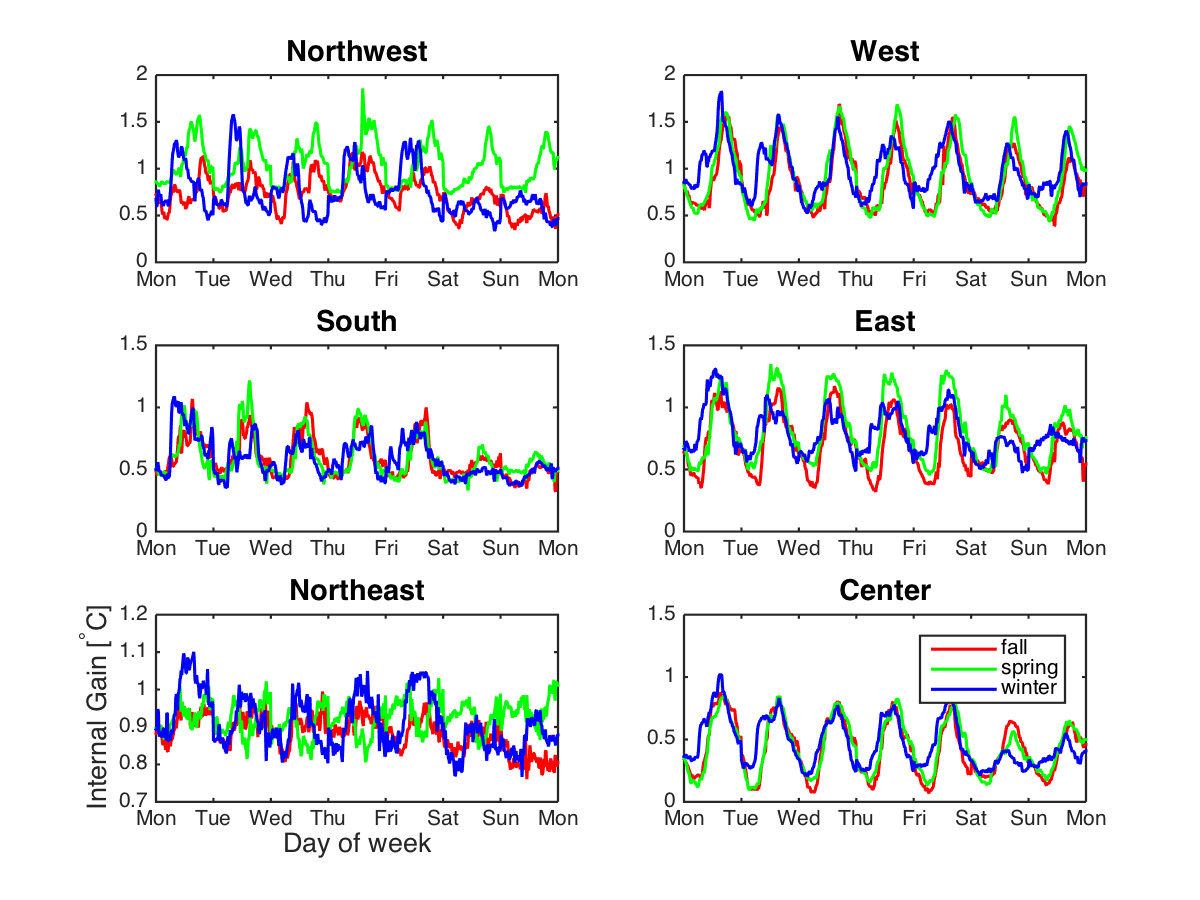
\includegraphics[width=\textwidth]{chapters/building_model/figures/physics_qig.png}
	\vspace*{-0.2cm}
	\caption{Estimated Internal Gain $f_{\text{IG}}$ from the Physics-Based Model by Zone and Season}
	\vspace*{-0.5cm}
	\label{fig:physics_qig}
\end{figure}
%!TEX root = ../../thesis.tex

\section{Quantitative Comparison of both Models}
\label{sec:Comparison}

\subsection{Prediction Accuracy}\label{sec:prediction_accuracy}
The high-dimensional physics-based model (Model B) is found to have a higher prediction accuracy compared to the low-dimensional data-driven model for the individual zones (Model A) presented in Section \ref{sec:Indiv_Zones}: According to Table \ref{tab:data_RMS_zones}, the mean RMS error for Model B across zones is $0.11^\circ \text{C}$ lower than for Model A. This is also illustrated in Figure \ref{fig:open_loop_trajectories}, which shows 7-day open-loop predictions of the temperature of a randomly selected holdout test week in the spring period, simulated with both models initialized with the measured temperature. The increase in RMS error from Model B to Model A is notably larger in the zones ``East'' (0.38) and ``Center'' (0.15), compared to the other zones (0.11, $-$0.03, 0.07, and 0.08). 

This provides new insight into the existing knowledge as we provide a quantitative comparison between the low-dimensional data-driven model and the high-dimensional physics-based model's prediction accuracy for the same multi-zone commercial building, which is in regular operation. The existing literature merely mentions that data-driven models are likely to have lower prediction accuracies than physics-based ones and, to the best of our knowledge, a quantitative comparison at this level is non-existent, as previous building models were developed for different testbeds, fictitious buildings or from simulated data.
%We show what prediction accuracies are achievable by each model when applied to a building subjected to disturbances such as occupancy, without using additional hardware such as occupancy sensors.

Next, we explore the extent to which this slightly lower prediction accuracy of Model A affects its resulting controller's closed-loop performance in a building energy efficiency example.

\begin{table}[hbtp]
\centering
\begin{tabular}{*8c}
\toprule
\multicolumn{8}{c}{Data-Driven Model} \\
\hline
Season & NW & W & S & E & NE & C & Mean \\ \hline
Fall & 0.98 & 0.61 & 0.28 & 0.42 & 0.28 & 0.36 & 0.488\\
Winter & 1.41 & 0.34 & 0.29 & 0.26 & 0.25 & 0.21 & 0.460\\
Spring & 0.56 & 0.25 & 0.31 & 0.71 & 0.17 & 0.34 & 0.390\\
\midrule
\midrule
\multicolumn{8}{c}{Physics-Based Model} \\
\hline
Season & NW & W & S & E & NE & C & Mean \\ \hline
Fall & 0.61 & 0.46 & 0.39 & 0.39 & 0.20 & 0.32 & 0.396\\
Winter & 0.55 & 0.39 & 0.34 & 0.32 & 0.18 & 0.24 & 0.338\\
Spring & 0.45 & 0.28 & 0.24 & 0.33 & 0.09 & 0.19 & 0.263\\
\bottomrule
\end{tabular}
\caption{RMS by Zone and Season for Data-Driven and Physics-Based Models}
\label{tab:data_RMS_zones}
\end{table}



\begin{figure}
\centering
\vspace*{-0.1cm}
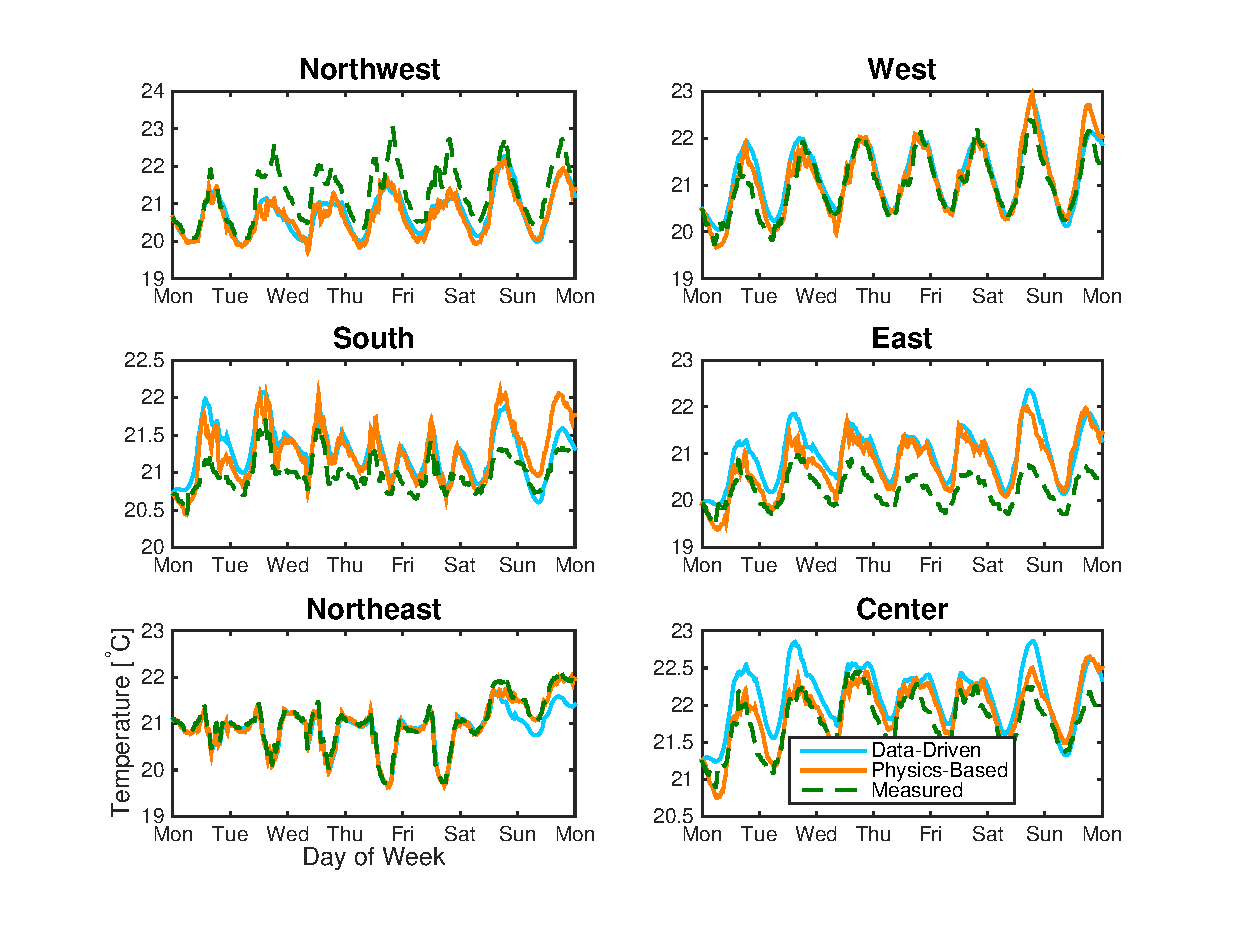
\includegraphics[width=\textwidth]{chapters/building_model/figures/open_loop_traj.eps}
\vspace*{-0.5cm}
\caption{Simulated Temperatures from the Data-Driven Model (blue), Physics-Based Model (orange) and Actual Temperatures (green) }
\vspace*{-0.5cm}
\label{fig:open_loop_trajectories}
\end{figure}
%The higher inaccuracy of the data-driven model becomes particularly apparent in zones Center and East, where the data-driven estimate notably deviates from the measured temperatures.

\subsection{Energy Efficient Control}\label{sec:energy_efficient_control}
In this section, we compare the performance of Model A and Model B for the purpose of energy efficiency. We formulate an MPC problem to find the optimal control strategy that minimizes the cost of HVAC operation over the same week used in Figure \ref{fig:open_loop_trajectories}, while guaranteeing the temperature to stay within a comfort zone $[T_{\text{min}}, T_{\text{max}}]$, which we chose as $[20^\circ \text{C}, 22^\circ \text{C}]$ \cite{Hansen:2013aa}, and confining the control input to the physical limits of the HVAC system $[u_{\text{min}}, u_{\text{max}}]$. This problem is formulated as follows:
\begin{equation}\label{eq:ee_controller}
\begin{split}
\min_{u, \varepsilon}~&\sum_{k=1}^N u(k)^2 + \rho \Vert\varepsilon\Vert_2 \\
\text{s.t.}~& x(0) = \bar{x}(0) \\
& x(k+1) = \begin{cases}
      \eqref{eq:temp_propagation_indiv}, & \text{Model A}  \\
      \eqref{eq:physics_model1}, & \text{Model B}
    \end{cases} \\
& u_{\text{min}}-\varepsilon \leq u(k) \leq u_{\text{max}}+\varepsilon\qquad \forall k\in[0, N-1]\\
& \begin{cases}
      T_{\text{min}} \leq x(k) \leq T_{\text{max}}, & \text{Model A}  \\
      T_{\text{min}} \leq Cx(k) \leq T_{\text{max}}, & \text{Model B}~\eqref{eq:physics_model_2}
    \end{cases}~ \forall k\in[1, N]
\end{split}
\end{equation}
The temperature is initialized with the measured temperature $\bar{x}(0)$ at the beginning of the week-long simulation. We use soft constraints on the control input with a penalty parameter $\rho$ to ensure the feasibility of the problem. The penalty represents the cost of increasing the airflow beyond the operating limits (temporary shutdown or overuse, both of which are harmful to the system). 
%The function $f(x(\cdot), u(\cdot), v(\cdot), q_{\text{IG}}(\cdot))$ is chosen to be either \eqref{eq:temp_propagation_indiv} for Model A or\eqref{eq:physics_model} for Model B.
To find the optimal control strategy, we make use of receding horizon control with a prediction horizon of three 15-minute time steps.


\begin{figure}
\centering
\vspace*{-0.4cm}
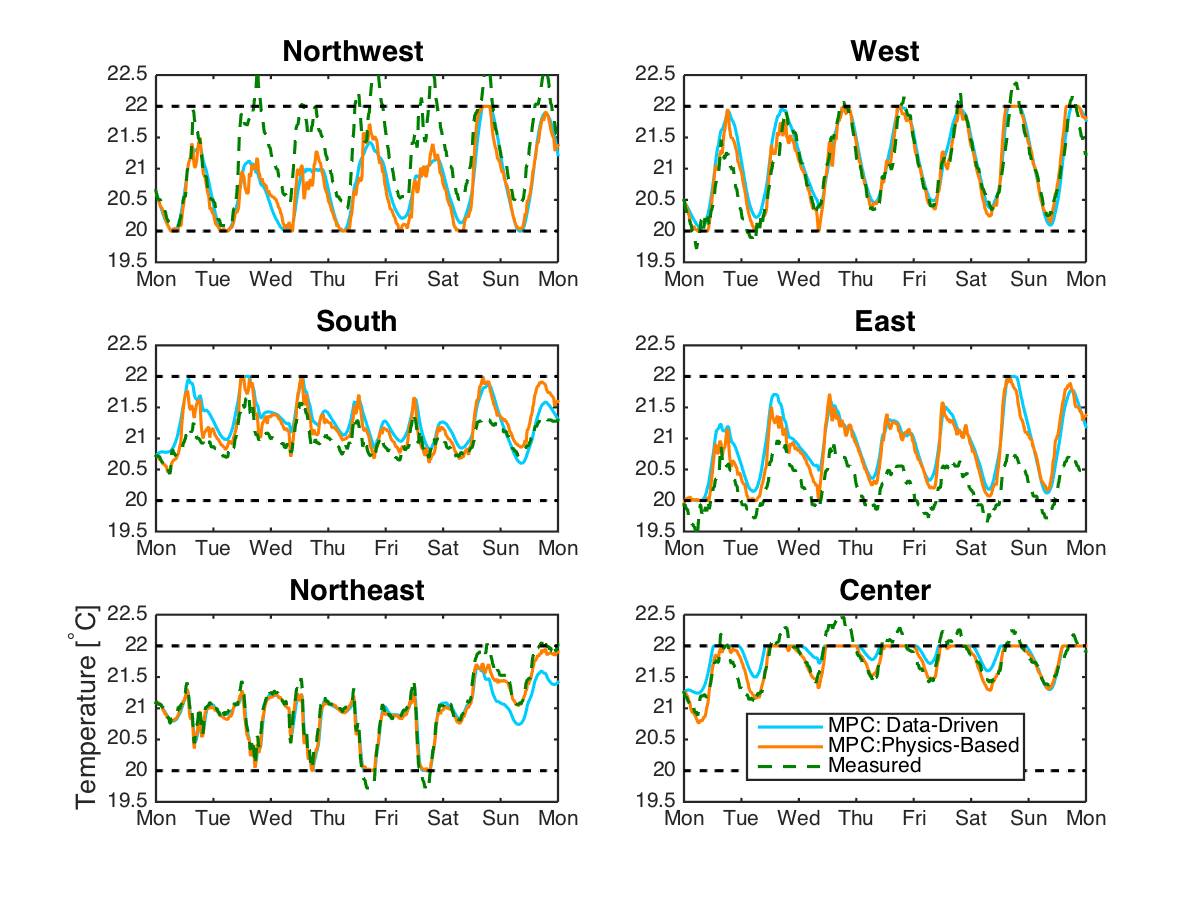
\includegraphics[width=\textwidth]{chapters/building_model/figures/Comparison_Temp.png}
\vspace*{-0.5cm}
\caption{Optimal Temperature for MPC with Data-Driven Model (blue), MPC with Physics-Based Model (orange) and Actual Temperature (green)}
\vspace*{-0.2cm}
\label{fig:MPC_comparison_temp}
\end{figure}

\begin{figure}
\centering
%\vspace*{-0.4cm}
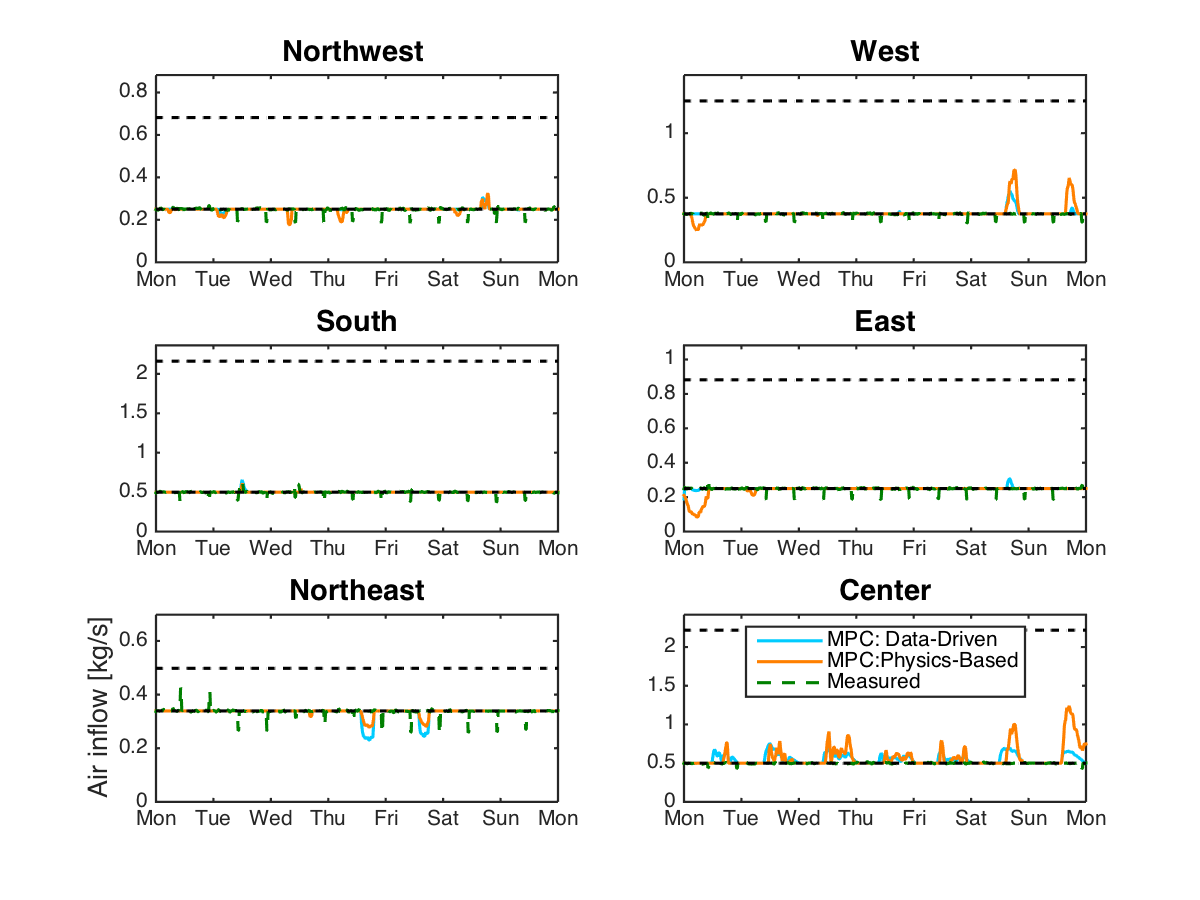
\includegraphics[width=\textwidth]{chapters/building_model/figures/Comparison_Flow.png}
\vspace*{-0.5cm}
\caption{Optimal Control Strategy for MPC with Data-Driven Model (blue), MPC with Physics-Based Model (orange) and Actual Input (green)}
%\vspace*{-0.2cm}
\label{fig:MPC_comparison_flow}
\end{figure}

Figure \ref{fig:MPC_comparison_temp} shows the temperature trajectory computed by the energy efficient controller \eqref{eq:ee_controller} computed with both models A and B, together with the measured temperature as a reference. 
It can be seen that both control schemes are capable of maintaining the temperature within $[20^\circ \text{C}, 22^\circ \text{C}]$, with a control strategy that is of comparable cost (1,006 and 1,731 for Model A and Model B, respectively, where $\rho=100$), shown in Figure \ref{fig:MPC_comparison_flow}. An interesting observation is that the largest difference in the control strategies is detected in zones ``East'' and ``Center'', which show a larger increase in RMS error from Model B to Model A.
%The dips of the computed control trajectory $u$ below the black dashed lines represent violations of the physical limits needed to maintain the temperature in the narrow range $[20^\circ, 22^\circ]$. 
Furthermore, it is interesting to observe that variations in the control input do not impact the periodicity of the temperature qualitatively, which can be explained by the regularity of the identified internal gains.

These findings suggest that both models perform equally well in designing an energy efficient control strategy. However, computing this strategy for Model A was cheap ($<5$ minutes) compared to Model B ($\approx 20$ hours) on a 2 GHz Intel Core i7, 16 GB 1600 MHz DDR3 machine. Further, we note that in real-world applications, the MPC would use state feedback to initialize the temperature with sensor measurements at every time step, whereas in our simulation, it operates in an ``open loop'' fashion and hence propagates the estimation error with time. This will reduce the difference in the prediction quality by both controllers even further, since the RMS error is now to be evaluated on a much shorter prediction horizon, thereby further corroborating the finding of almost identical control schemes.

Observing that Model A only suffers a negligible loss of accuracy compared to Model B for an open loop optimal control scheme, our findings suggest the applicability of Model A to other applications with temperature-critical zones in which even more precise temperature estimates are needed, e.g. long-term planning of reserve provision for frequency regulation.

%\textcolor{red}{While our findings suggest that Model A is suitable for tasks that can tolerate minor inaccuracies, such as energy efficient control, we note that for temperature-critical zones or applications in which precise temperature estimates are needed, e.g. long-term planning of reserve provision for frequency regulation, one might still want to choose the fine-level Model B for analysis.}



%%%%%%%%%%%%%%%%%%
%\subsection{Qualitative Comparison}
%We summarize the findings in the following:
%\begin{itemize}
%\item Model A is more \textit{amenable} to controller design due to its low dimensionality and hence considerably faster operation. This is of particular importance for \textit{scalability} considerations, since the computation time grows exponentially with the number of state variables, which renders Model B computationally intractable for online operation beyond a certain complexity. Indeed we observe that the computation for one step of \eqref{eq:ee_controller} exceeds 15 minutes $-$ the discretization time $-$ for a prediction horizon of five steps. Thus in frequency regulation, for instance, Model A's low dimensionality makes it suitable for reserve determination which must be computed for a time horizon of 24 hours.
%\item Identifying Model A with semiparametric regression only relies on temperature and VAV airflow data and the physical adjacency of zones, in contrast to Model B, which requires knowledge of the BRCM toolbox and a large amount of geometry and construction data of the buildings, many of which are often unknown \cite{Qie}. Hence, more effort is required to train the model on new buildings for Model B.
%\item The higher \textit{accuracy} of Model B proves useful for applications such as the control of temperature-critical zones and evaluation of controller performance through simulations, whereas Model A is preferably used for controller design and in applications where less emphasis is put on estimation errors, e.g. at night when building occupancy is low. 
%\item Model A assumes a uniform temperature among zones, which often encompass several rooms, whereas Model B can provide estimates for the temperature of individual rooms in a given zone. The number of parameters of Model A increases rapidly with the model complexity, which coupled with insufficient excitation of the system makes it hard to emulate the higher spatial \textit{granularity} with Model A. 
%\end{itemize}

%With a negligible contribution of $\mathbf{c}\cdot\mathbf{w}$ on the temperature evolution, equation \eqref{eq:Temperature_evolution} becomes
%\begin{equation}\label{eq:temp_evolution_decomp}
%x(n+1) = a x(n) + b u(n) + q_{\text{IG}}(n).
%\end{equation}
%As mentioned before, the main problem in the identification of the true physical value of $b$ lies in the lack of sufficient excitation of the temperature dynamics. Inspired by the prior knowledge of the VAV airflow, we chose $\hat{b}$ to be close to the approximated prior. For a fixed value of $\hat{b}$, the value of $\hat{a}$ minimizing the mean RMS is found to be $\approx 0.85$. Thus, fixing $a=0.85$, the only variable terms in \eqref{eq:temp_evolution_decomp} become $b u(n)$ and $q_{\text{IG}}$, and we thus obtain
%\begin{equation}
%\begin{aligned}
%0 &= \left(\hat{b}-b_{\text{opt}}\right)u(n) + \left(\hat{q}_{\text{IG}} - q_{\text{IG}}^{\text{opt}} \right)\\
%\hat{q}_{\text{IG}}(n) &= q_{\text{IG}}^{\text{opt}}(n) - \left(\hat{b}-b_{\text{opt}}\right)u(n)
%\end{aligned}
%\end{equation}
%by subtracting \eqref{eq:temp_evolution_decomp} for the optimal $b_{\text{opt}} = -0.03$ from \eqref{eq:temp_evolution_decomp} for the a-priori defined value $\hat{b} = -0.18$. We therefore find that different values of the estimated parameter $b$ result in a shift of the estimated internal gain. Further, we conclude that the internal gain estimated by the data-driven approach consists of two main contributions: the exogenous heating load due to occupancy and electric devices $q_{\text{exo}}$ (constant for a different season with weekly seasonality) and a variable term $q_{\text{bal}}$ that balances varying levels of the control input effect $|b\cdot u|$:
%\begin{equation}\label{eq:IG_decomposition}
%q_{\text{IG}}(n) = q_{\text{exo}}(n) + q_{\text{bal}}(n).
%\end{equation}
%Therefore the physically meaningful gain due to occupancy and electric devices $q_{\text{exo}}$ is masked and cannot be isolated from \eqref{eq:IG_decomposition}. It follows that different levels of internal gains for the different seasons (Figure \ref{fig:data_lump_qig} can only be assessed on a relative level
%
%In contrast to the data-driven approach, the physics-based model is able to isolate the exogenous occupancy load ...
%!TEX root = ../../thesis.tex

\section{Conclusion}
\label{sec:Conclusion}

We identified two state-space models for the thermal behavior of the same multi-zone commercial building using experimental data collected during regular building operation. One of the models is a low-dimensional data-driven model identified using semiparametric regression, the other one is a high-dimensional physics-based resistance-capacitance model. Both models capture the effect of disturbances such as occupancy and electrical appliances that commercial buildings are subjected to, without installation of any additional hardware such as occupancy sensors. 

The identification of both models on the \textit{same building} enabled us to quantitatively compare the performance of these types of models when applied to a real building, which has not been done before. Our results showed that the RMS error of the open-loop temperature prediction of the physics-based model across different thermal zones and temporal seasons is $0.11^\circ \text{C}$ lower than in the data-driven model, a $25\%$ reduction. However, simulating energy efficient MPC schemes under both models suggested both models perform equally well in terms of cost function minimization and constraint satisfaction despite the significantly higher complexity of the physics-based model.

%However is this improvement significant in closed-loop control schemes? To answer this question, we simulated energy efficient MPC schemes for both models on this building, and concluded that the models performed equally well in terms of cost function minimization and constraint satisfaction. However, as expected, the physics-based model was computationally more expensive due to its large number of states and its bilinear nature. 

It is widely known in this field that low-dimensional data-driven models have lower prediction accuracy than high-dimensional physics-based models, and thus have been only proposed for control of less temperature-critical buildings or zones. However, our work investigated an identification method for data-driven models for multi-zone commercial buildings in regular operation and demonstrated that the lower open-loop prediction accuracy of such data-driven models is insignificant in closed-loop control schemes compared to a high-dimensional physics-based model. Based on these findings, we suggest that such data-driven models may be suitable for applications that were previously considered inappropriate, e.g. frequency regulation.

%We identified state-space models for the thermal behavior of SDH with semiparametric regression and a physics-based model on the \textit{same} testbed. The internal gains due to occupants and electric devices were identified for different spatial granularities and different temporal seasons. We found the high-dimensional physics-based model to yield lower estimation errors than the low-dimensional data-driven model due to the inclusion of analytical temperature models based on physical parameters of the building, therefore allowing for higher granularity in temperature predictions. Under an energy efficient MPC scheme, however, both models performed equally well, with the disadvantage of the physics-based model being computationally expensive due to its large number of states that are bilinearly related with inputs.

%We note that the higher fidelity physics-based model should be used for controlling temperature-critical zones in buildings, since it provides higher granularity in addition to higher accuracy. The compact data-driven model, however, is a good alternative for devising a control strategy when less emphasis is put on estimation errors, e.g. at night when occupancy is low. In frequency regulation, the lower-dimensional data-driven model is more suitable for reserve determination as it requires planning over a longer time horizon, whereas the more accurate higher-dimensional physics-based model can be used in reserve provision to maintain the building temperature within comfort bounds and track the frequency regulation signal. Furthermore, while semiparametric regression can be easily applied on any building with a modest requirement of recorded data, the physics-based model requires detailed geometry and construction data about the building, which in practice is often subject to large inaccuracies, and therefore hard to obtain.

%Finally, we are currently working on verifying our hypothesis by designing and implementing a control scheme suitable for frequency regulation, using the data-driven model, into the building operation system of SDH.


